\documentclass[conference]{IEEEtran}
\IEEEoverridecommandlockouts
% The preceding line is only needed to identify funding in the first footnote. If that is unneeded, please comment it out.
\usepackage{cite}
\usepackage{amsmath,amssymb,amsfonts}
\usepackage{algorithmic}
\usepackage{graphicx}
\usepackage{textcomp}
\usepackage[ruled]{algorithm2e} % For algorithms
\usepackage{caption}
\usepackage{subcaption}
\usepackage{color}
\usepackage{multirow}

\def\BibTeX{{\rm B\kern-.05em{\sc i\kern-.025em b}\kern-.08em
    T\kern-.1667em\lower.7ex\hbox{E}\kern-.125emX}}
\begin{document}

\title{Time Series Deinterleaving with Application in Malicious Domain Detection\\
\thanks{Identify applicable funding agency here. If none, delete this.}
}





\author{\IEEEauthorblockN{Amir Asiaee T.}
\IEEEauthorblockA{\textit{Mathematical Biosciences Institute} \\
\textit{Ohio State University}\\
Columbus, OH\\
asiaeetaheri.1@osu.edu}
\and
\IEEEauthorblockN{Hardik Goel}
\IEEEauthorblockA{\textit{} \\
\textit{Microsoft Corporation}\\
Redmond, Washington\\
hagoel@microsoft.com}
\and
\IEEEauthorblockN{Vinod Yegneswaran}
\IEEEauthorblockA{\textit{Computer Science Laboratory} \\
	\textit{SRI International}\\
	Menlo Park, CA \\
	vinod@csl.sri.com}
\and
\IEEEauthorblockN{Shalini Ghosh}
\IEEEauthorblockA{\textit{Computer Science Laboratory} \\
\textit{SRI International}\\
Menlo Park, CA\\
shalini@csl.sri.com}
\and
\IEEEauthorblockN{Arindam Banerjee}
\IEEEauthorblockA{\textit{Department of Computer Science} \\
\textit{University of Minnesota}\\
Minneapolis, MN\\
banerjee@cs.umn.edu}
}
\newcommand{\norm}[2]{\|#1\|_{#2}}
\newcommand{\kl}{D_{\text{KL}}}
\newcommand{\vl}{\text{Vol}}

\newcommand{\beq}{\begin{equation}}
\newcommand{\eeq}{\end{equation}}

\newcommand{\htn}{\hat{\theta}_{\lambda_n}}
\newcommand{\hdn}{\hat{\Delta}_n}


%% ========================================================
\newcommand\B{\mathbb{B}}
\newcommand\E{\mathbf{E}}
%\newcommand\I{\mathbb{I}}
\newcommand\N{\mathbb{N}}
\renewcommand\O{\mathbf{O}}
\renewcommand\P{\mathbf{P}}
\newcommand\Q{\mathbf{Q}}
\renewcommand\S{\mathbb{S}}
\newcommand\R{\mathbb{R}}
\newcommand\T{\mathbf{T}}
\newcommand\W{\mathbb{W}}
%\newcommand\X{\mathbb{X}}
\newcommand\Y{\mathbb{Y}}

\newcommand\1{\mathbbm{1}}
\newcommand\0{\mathbbm{0}}

\newenvironment{packed_enum}{
	\begin{enumerate}
		\setlength{\itemsep}{1pt}
		\setlength{\parskip}{0pt}
		\setlength{\parsep}{0pt}
	}{\end{enumerate}}

%% ========================================================
%% Some useful commands. Note the dangerous \r command!
%% ========================================================



\newcommand{\bd}{\boldsymbol}
\newcommand{\mf}{\mathbf}


\newcommand{\g}{\mathbf{g}}

\renewcommand{\a}{\mathbf{a}}
\renewcommand{\c}{\mathbf{c}}
\newcommand{\e}{\mathbf{e}}
\newcommand{\f}{\mathbf{f}}
\renewcommand{\r}{\mathbf{r}} % since \r was already defined in altex
\renewcommand{\u}{\mathbf{u}}
\renewcommand{\v}{\mathbf{v}}
\renewcommand{\o}{\mathbf{o}}
\newcommand{\s}{\mathbf{s}}
\newcommand{\w}{\mathbf{w}}
\newcommand{\x}{\mathbf{x}}
\newcommand{\y}{\mathbf{y}}
\newcommand{\z}{\mathbf{z}}
\newcommand{\p}{\mathbf{p}}
\newcommand{\q}{\mathbf{q}}

\newcommand\X{\mathbf{X}}
\newcommand\A{\mathbf{A}}
\newcommand\I{\mathbf{I}}


%----------------------------------------
%      THE SETS
%----------------------------------------
\newcommand{\cC}{{\cal C}}
\newcommand{\cH}{{\cal H}}
\newcommand{\cK}{{\cal K}}
\newcommand{\cL}{{\cal L}}
\newcommand{\cM}{{\cal M}}
\newcommand{\cN}{{\cal N}}
\newcommand{\cP}{{\cal P}}
\newcommand{\cQ}{{\cal Q}}
\newcommand{\cS}{{\cal S}}
\newcommand{\cT}{{\cal T}}
\newcommand{\cV}{{\cal V}}
\newcommand{\cX}{{\cal X}}
\newcommand{\cY}{{\cal Y}}
\newcommand{\cF}{{\cal F}}
\newcommand{\cZ}{{\cal Z}}


%--------------------------------------------
%         THE VARIABLES & APPROXIMATES
%--------------------------------------------

% Bold variables for vectors, matrices
\newcommand{\bA}{\mathbf{A}}
\newcommand{\bB}{\mathbf{B}}
\newcommand{\bC}{\mathbf{C}}
\newcommand{\bD}{\mathbf{D}}
\newcommand{\bE}{\mathbf{E}}
\newcommand{\bI}{\mathbf{I}}
\newcommand{\bM}{\mathbf{M}}
\newcommand{\bP}{\mathbf{P}}
\newcommand{\bQ}{\mathbf{Q}}
\newcommand{\bR}{\mathbf{R}}
\newcommand{\bU}{\mathbf{U}}
\newcommand{\bV}{\mathbf{V}}
\newcommand{\bW}{\mathbf{W}}
\newcommand{\bX}{\mathbf{X}}
\newcommand{\bY}{\mathbf{Y}}
\newcommand{\bZ}{\mathbf{Z}}

\newcommand{\bz}{\mathbf{z}}
\newcommand{\hZ}{\hat{Z}}
\newcommand{\hbZ}{\hat{\bZ}}
\newcommand{\hz}{\hat{z}}

\newcommand{\hU}{\hat{U}}
\newcommand{\hV}{\hat{V}}
\newcommand{\hu}{\hat{u}}
\newcommand{\hv}{\hat{v}}
\newcommand{\htth}{\hat{\ttheta}}


\newcommand{\pr}{\mathbb{P}}
\newcommand{\ex}{\mathbb{E}}


\newcommand{\hX}{\hat{X}}
\newcommand{\hY}{\hat{Y}}
\newcommand{\hatx}{{\hat{x}}}
\newcommand{\haty}{{\hat{y}}}

%---------MISC-----------------------------

\newcommand{\vertiii}[1]{{\left\vert\kern-0.25ex\left\vert\kern-0.25ex\left\vert #1
		\right\vert\kern-0.25ex\right\vert\kern-0.25ex\right\vert}}

\newcommand{\BNi}{\bB_N^{(i)}}
\newcommand{\xai}{\x_i^{(a)}}
\newcommand{\yai}{\bY_i^{(i)}}
\newcommand{\Xai}{\bX_i^{(a)}}
\newcommand{\Yai}{\bY_i^{(i)}}


\newcommand{\m}{\boldsymbol{\mu}}
\newcommand{\llambda}{\boldsymbol{\lambda}}
\newcommand{\xx}{\boldsymbol{\chi}}
\newcommand{\Th}{\boldsymbol{\theta}}
\newcommand{\Eta}{\boldsymbol{\eta}}
\newcommand{\oomega}{\boldsymbol{\omega}}
\newcommand{\ppi}{\boldsymbol{\pi}}
\newcommand{\pphi}{\boldsymbol{\phi}}
\newcommand{\ggamma}{\boldsymbol{\gamma}}
\newcommand{\bbeta}{\boldsymbol{\beta}}
\newcommand{\aalpha}{\boldsymbol{\alpha}}
\newcommand{\ttheta}{\boldsymbol{\theta}}
\newcommand{\eepsilon}{\boldsymbol{\epsilon}}
%\newcommand{\norm}[2]{\ensuremath \|#1\|_{#2}}
\newcommand{\no}[1]{\norm{#1}{}}
\newcommand{\myref}[1]{(\ref{#1})}
\newcommand{\del}[2]{\frac{\partial #1}{\partial #2}}


%----------------------------------------------
%        NEW OPERATORS
%----------------------------------------------
%\DeclareMathOperator*{\argmax}{\arg\!\max}
%\DeclareMathOperator*{\argmin}{\arg\!\min}
%\DeclareMathOperator{\avg}{avg}
%\DeclareMathOperator{\Int}{int}
%\DeclareMathOperator{\cl}{cl}
%\DeclareMathOperator{\bnd}{bd}
%\DeclareMathOperator{\epi}{epi}
%\DeclareMathOperator{\dom}{dom}
%\DeclareMathOperator{\ri}{ri}
%\DeclareMathOperator{\co}{co}
%\DeclareMathOperator{\sgn}{sign}
%\DeclareMathOperator{\supp}{supp}
%\DeclareMathOperator{\discrete}{Discrete}
%\DeclareMathOperator{\gam}{GAM}
%\DeclareMathOperator{\uni}{Uniform}
%\DeclareMathOperator{\dir}{Dir}
%\DeclareMathOperator{\gaam}{GAM}
%\DeclareMathOperator{\Beta}{Beta}
%\DeclareMathOperator{\tr}{Tr}
%\DeclareMathOperator{\cone}{cone}

%---------------------------------------------
% EQUATION, FIGURE, TABLE NUMBERS
%---------------------------------------------

%\renewcommand{\theequation}{\thesection.\arabic{equation}}
%\renewcommand{\thefigure}{\thesection.\arabic{figure}}
%\renewcommand{\thetable}{\thesection.\arabic{table}}
%\numberwithin{equation}{section}



%---------------------------------------------
% THEOREMS, EXAMPLES ETC.
%---------------------------------------------
%
%\newcounter{exampleI}
%\setcounter{exampleI}{1}
%\renewcommand{\theexampleI}{\arabic{exampleI}}
%
%{\theorembodyfont{\rmfamily} \theoremstyle{plain} \newtheorem{subexampleI}{Example}[exampleI]}
%\renewcommand{\thesubexampleI}{\theexampleI.\Alph{subexampleI}}
%
%\newcounter{exampleII}
%\setcounter{exampleII}{2}
%\renewcommand{\theexampleII}{\arabic{exampleII}}
%
%{\theorembodyfont{\rmfamily} \theoremstyle{plain} \newtheorem{subexampleII}{Example}[exampleII]}
%\renewcommand{\thesubexampleII}{\theexampleII.\Alph{subexampleII}}
%
%\newcounter{exampleIII}
%\setcounter{exampleIII}{3}
%\renewcommand{\theexampleIII}{\arabic{exampleIII}}
%
%{\theorembodyfont{\rmfamily} \theoremstyle{plain} \newtheorem{subexampleIII}{Example}[exampleIII]}
%\renewcommand{\thesubexampleIII}{\theexampleIII.\Alph{subexampleIII}}
%
%
%{\theorembodyfont{\rmfamily} \newtheorem{exm}{Example}}
%{\theorembodyfont{\rmfamily} \newtheorem{defn}{Definition}}
%%{\theorembodyfont{\rmfamily} \newtheorem{remark}{Remark}}
%\newtheorem{theo}{Theorem}
\newtheorem{prop}{Proposition}
\newtheorem{lemm}{Lemma}
\newtheorem{corr}{Corollary}
\newtheorem{clm}{Claim}
%\newcommand{\proof}{\noindent{\itshape Proof:}\hspace*{1em}}
\newcommand{\proofsketch}{\noindent{\itshape Proof Sketch:}\hspace*{1em}}
%\newcommand{\qed}{\nolinebreak[1]~~~\hspace*{\fill} \rule{5pt}{5pt}\vspace*{\parskip}\vspace*{1ex}}



\newcommand{\cx}{{\hat{x}}}
\newcommand{\cy}{{\hat{y}}}
\newcommand{\bp}{{\bar{p}}}
\newcommand{\eqn}[1]{(\ref{eq:#1})}
\newcommand {\commentout}[1] {}

%------------------------------------------

%%%%%%%%%%%Definitions and Macros

\def\ints{{{\rm Z} \kern -.35em {\rm Z} }}  % ints
\def\smallints{{{\rm Z} \kern -.3em {\rm Z} }}  % small ints
\def\pints{{{\rm I} \kern -.15em {\rm N} }}      % pints
\newcommand{\reals}{\mathbb R}
\newcommand{\naturals}{\mathbb N}
\newcommand{\integers}{\mathbb Z}

\newcommand{\lapn}{\lessapprox_{\,n}}
\newcommand{\gapn}{\gtrapprox_{\,n}}
\newcommand{\apn}{\approx_n}

%\def\reals{{{\rm I} \kern -.2em {\rm R} }} % reals
\newcommand{\RR}{\mathbb R}
\def\cplx{{{\rm I} \kern -.45em {\rm C} }}       % complex
\def\l2{\rm {\mathcal L}^{2}(\reals)}            % l2

\newcommand{\seqz}[2]{\mbox{$\{#1_{#2}\}$}_{#2 \in \smallints }}
\newcommand{\seqn}[2]{\mbox{$\{#1_{#2}\}$}_{#2 \in \pints }}
%\renewcommand{\norm}[1]{\lVert#1\rVert}
\newcommand{\abs}[1]{\left|#1\right|}


%\newtheorem{problem}{Problem}
%\newtheorem{definition}{Definition}[section]
%\newtheorem{nad}{Notation and Definitions}[section]
%\newtheorem{notation}{Notation}[section]
%\newtheorem{remark}{Remark}[section]
%\newtheorem{theorem}{Theorem}[section]
%\newtheorem{lemma}[theorem]{Lemma}
%\newtheorem{claim}{Claim}[theorem]
%\newtheorem{proposition}{Proposition}[section]
%\newtheorem{corollary}{Corollary}
%\newtheorem{example}{Example}
%\newtheorem{conjecture}{Conjecture}
%\newtheorem{algorithm}{Algorithm}
%\newtheorem{exercise}{Exercise}
%\newtheorem{step}{Step}

\newcommand{\nr}{\nonumber}
\newcommand{\be}{\begin{eqnarray}}
\newcommand{\ee}{\end{eqnarray}}
\newcommand{\bea}{\begin{eqnarray}}
\newcommand{\eea}{\end{eqnarray}}
\newcommand{\beaa}{\begin{eqnarray*}}
	\newcommand{\eeaa}{\end{eqnarray*}}
\newcommand{\bnad}{\begin{nad}}
	\newcommand{\enad}{\end{nad}}


\newcommand{\gb}{\beta_{\infty}}
\newcommand{\mgb}{\tilde{\beta}_{\infty}}
\newcommand{\gbb}{\beta_{2}}
\newcommand{\mgbb}{\tilde{\beta}_{2}}
\newcommand{\Jf}{J_{\infty}}
\newcommand{\mmJf}{\overline{J}_{\infty}}
\newcommand{\mJf}{\tilde{J}_{\infty}}
\newcommand{\Jff}{J_{2}}
\newcommand{\mJff}{\tilde{J}_{2}}
\newcommand{\Jc}{{\calJ_{\infty}}}
\newcommand{\mJc}{{\tilde{\calJ}_{\infty}}}
\newcommand{\Jcc}{{\calJ_{2}}}
\newcommand{\ptq}{P_{3 \overline{Q}}}
\newcommand{\pq}{P_{Q}}


\newcommand{\di}{{\,\mathrm{d}}}
\newcommand{\latop}[2]{\genfrac{}{}{0pt}{}{#1}{#2}}


%\newcommand{\Th}[1]{Theorem~\ref{#1}} % when starting a sentence
%\renewcommand{\th}[1]{Theorem~\ref{#1}}
%\newcommand{\ths}[2]{Theorems~\ref{#1} and~\ref{#2}}
%\newcommand{\thst}[2]{Theorems~\ref{#1}-\ref{#2}}
%\newcommand{\lem}[1]{Lemma~\ref{#1}}
%\newcommand{\prop}[1]{Proposition~\ref{#1}}
%\newcommand{\defin}[1]{Definition~\ref{#1}}
%\newcommand{\eq}[1]{equation~(\ref{#1})}
%\newcommand{\ineq}[1]{inequality~(\ref{#1})}
%\newcommand{\Ineq}[1]{Inequality~(\ref{#1})}
%\newcommand{\ineqs}[2]{inequalities~(\ref{#1}) and~(\ref{#2})}
%\newcommand{\Eq}[1]{Equation~(\ref{#1})}
%\newcommand{\eqs}[2]{equations~(\ref{#1}) and~(\ref{#2})}
%\newcommand{\eqss}[3]{equations~(\ref{#1}), (\ref{#2}) and~(\ref{#3})}
%\newcommand{\eqst}[2]{equations~(\ref{#1})-(\ref{#2})}
%\newcommand{\sect}[1]{Section~\ref{#1}}
%\newcommand{\subsect}[1]{Subsection~\ref{#1}}

\newcommand{\lip}{\langle}
\newcommand{\rip}{\rangle}
\newcommand{\uu}{\underline}
\newcommand{\oo}{\overline}
\newcommand{\La}{\Lambda}
\newcommand{\la}{\lambda}
%\newcommand{\eps}{\epsilon}
\newcommand{\eps}{\varepsilon}
\newcommand{\veps}{\varepsilon}
\newcommand{\rmT}{{\rm T}}
\newcommand{\rmW}{{\rm W}}
\newcommand{\Ga}{\Gamma}

\newcommand{\sign}{{\mbox{\rm sign}}}
\newcommand{\ang}{{\mbox{\rm ang}}}
%\newcommand{\supp}{{\mbox{\rm supp}}}
\newcommand{\dist}{{\mbox{\rm dist}}}

\newcommand{\nin}{\in\!\!\!\!\!/\,}

\newcommand{\calA}{{\cal A}}
\newcommand{\calB}{{\cal B}}
\newcommand{\calC}{{\cal C}}
\newcommand{\calD}{{\cal D}}
\newcommand{\tcD}{{\tilde{\cal D}}}
\newcommand{\calE}{{\cal E}}
\newcommand{\calF}{{\cal F}}
\newcommand{\calG}{{\cal G}}
\newcommand{\calH}{{\cal H}}
\newcommand{\calI}{{\cal I}}
\newcommand{\calJ}{{\cal J}}
\newcommand{\calK}{{\cal K}}
\newcommand{\calL}{{\cal L}}
\newcommand{\calM}{{\cal M}}
\newcommand{\calN}{{\cal N}}
\newcommand{\calO}{{\cal O}}
\newcommand{\calP}{{\cal P}}
\newcommand{\calQ}{{\cal Q}}
\newcommand{\calR}{{\cal R}}
\newcommand{\calS}{{\cal S}}
\newcommand{\calT}{{\cal T}}
\newcommand{\calU}{{\cal U}}
\newcommand{\calV}{{\cal V}}
\newcommand{\calW}{{\cal W}}
\newcommand{\calX}{{\cal X}}
\newcommand{\calY}{{\cal Y}}
\newcommand{\calZ}{{\cal Z}}

\newcommand{\RE}{{\cal R}e}
%\newcommand{\IM}{{\cal I}m}


\newcommand{\Prob}{{\rm Prob\,}}
\newcommand{\diam}{{\rm diam\,}}
\renewcommand{\mod}{{\rm mod\,}}
\newcommand{\sinc}{{\rm sinc\,}}
\newcommand{\ctg}{{\rm ctg\,}}
\newcommand{\ifff}{\mbox{\ if and only if\ }}
%\newcommand{\proof}{\noindent {\bf Proof:\ }}

%\renewcommand{\bar}{\overline}
\renewcommand{\overline}{\bar}
%\renewcommand{\tilde}{\widetilde}
\renewcommand{\widetilde}{\tilde}
%\renewcommand{\ell}{l}
%\renewcommand{\hat}{\widehat}
\renewcommand{\widehat}{\hat}


\newcommand{\boldx}{{\bf x}}
\newcommand{\boldX}{{\bf X}}
\newcommand{\boldy}{{\bf y}}
\newcommand{\indic}{{\large \bf 1}}
\newcommand{\uux}{\uu{x}}
\newcommand{\uuY}{\uu{Y}}

\newcommand{\opt}{\rm{opt}}


%fraction with round brackets
\newcommand{\ffrac}[2]
{\left( \frac{#1}{#2} \right)}

\newcommand{\one}{\frac{1}{n}\:}
\newcommand{\half}{\frac{1}{2}\:}


\newcommand{\BAMS}{{\em Bulletin of the Amer. Math. Soc.}}
\newcommand{\TAMS}{{\em Transactions of the Amer. Math. Soc.}}
\newcommand{\PAMS}{{\em Proceedings of the Amer. Math. Soc.}}
\newcommand{\JAMS}{{\em Journal of the Amer. Math. Soc.}}
\newcommand{\LNM}{{\em Lect. Notes in Math.}}
\newcommand{\LNCS}{{\em Lect. Notes in Comp. Sci.}}
\newcommand{\IV}{{\em Invent. Math.}}
\newcommand{\JAM}{{\em J. Anal. Math.}}
\newcommand{\Sc}{{\em Science}}


\maketitle

\begin{abstract}

Stream deinterleaving is an important problem with various
applications in the cybersecurity domain.  In this paper, we consider
the specific problem of deinterleaving DNS data streams using
machine-learning techniques, with the objective of automating the
extraction of malware domain sequences.  We first develop a generative model for
user request generation and DNS stream interleaving.  Based on these
we evaluate various inference strategies for deinterleaving including
augmented HMMs, RNNs and LSTMs on synthetic datasets.  Our results
demonstrate that state-of-the-art LSTMs outperform more traditional
RNNs and augmented HMMs in this application domain.
\end{abstract}
 

\begin{IEEEkeywords}
component, formatting, style, styling, insert
\end{IEEEkeywords}


		\section{Introduction}
	Deinterleaving temporal data streams is a general machine-learning
	problem with important applications to security and privacy.
	Specifically, interleaved network data streams are a common occurrence
	in cyber-threat monitoring which complicates many analyses.  In many
	instances, the individual stream identifiers are unavailable due
	to technical challenges, such as the vantage point of the data
	collector or are intentionally supressed to protect the privacy
	of the users in the network.
	
	For example, consider packet traces collected in a local area network,
	where the source IP addresses are removed or data collected from the
	external-facing interface of a proxy server or NAT firewall
	where individual client identifiers are unavailable.  Detecting anomalous
	behavior, especially stealthy and low-volume attack patterns, in
	these aggregated noisy streams is significantly more challenging than
	in a traditional deinterleaved setting.
	
	In this paper, we discuss a variant of this problem, i.e.,
	deinterleaving client request streams from recursive DNS resolvers
	to mine threat intelligence.  Such DNS data streams are shared
	among Internet service providers (ISPs) through mediums such
	as the Security Information Exchange (SIE) and are a valuable
	source of intelligence to the cybersecurity community.  Here, the individual
	client requests to the recursive DNS resolver are typically suppressed and
	what we have are inter-resolver communications (i.e, communications
	between the recursive resolver and the root server, TLD servers
	and other secondary resolvers).  We are interested in
	the application of advanced machine-learning techniques to automate
	the extraction of malware domain groups~\cite{} from such resolver streams.
	
	Malware infections while browsing the Internet have become very
	prevalent and occur due to various reasons such as drive-by exploits,
	phishing attacks etc.  In a typical infection, the user starts from
	a landing page and then goes through a sequence of seemingly harmless
	intermediate websites, until reaching a site that contains the malicious
	exploit that harm the user by installing malware or stealing private
	data.  The intermediate sites are typically redirection chains implemented
	in JavaScript for the purpose of obfuscation.
	Even though many landing and exploit websites are continously identified and
	blacklisted, thousands of new malicious domains emerge daily.  However,
	pieces of the redirection infrastructure get reused across campaigns
	and thus the actual sequence of websites traversed by the user contains
	information that may help in quickly identifying new exploit sites.
	
	When a user makes a browser request to visit a website, it first
	resolves the domain name by asking its recursive resolver.  If the
	answer for the query is cached by the resolver the answer is
	immediately provided to the client. Otherwise, it initiates a set of
	recursive queries, leading to the final queried website's IP address.
	Each webpage may have several embedded objects from many domains
	leading to a sequence of domain lookup requests emanating from the
	client.  Tracking the set of DNS requests made by each client is thus
	a useful means to identifying new and emergent malware infection
	sequences.  However, to protect user privacy ISPs typically only
	capture data from the external facing interface of the recursive
	resolver, effectively suppressing the individual client stream
	identifiers.  As there are hundreds of users making requests at the
	same period of time, and all of these requests are pushed to a single
	queue of a local DNS resolver, we cannot tell apart individual user's
	sequences of requests and perfectly deinterleaving all requests for
	deanonymization purposes is impossible.  However, our objective is not
	deanonymization, but rather extraction of malware domain sequences
	which are observed repeatedly across resolvers.  We believe that advanced
	machine learning strategies could be  in such selective
	deinterleaving of DNS time-series for the extraction of malware
	domain groups.
	
	
	{\bf Prior Work. } To the best of our knowledge deinterleaving has not
	been applied to DNS resolver queue's data.  Some earlier
	work \cite{gao2013empirical} investigates the use of a sliding window
	approach to identify new malicious domains by exploring the domains
	that typically form neighbors of known malicious domains in the
	resolver queue, while ignoring the actual sequential information.  The
	challenges of applying existing deinterleaving methods to DNS data is
	twofold.  First, most of the methods has been designed for
	deinterleaving Markov chains \cite{batu2004inferring,
		seroussi2009deinterleaving, seroussi2012deinterleaving,
		minot2014separation} and HMMs \cite{landwehr2008modeling}, and as we
	will discuss in Section~\ref{sec:gen}, the dynamics of submitting new queries to
	the local resolver is more complicated than simple Markov chain or
	HMM.  Moreover, the state space of the models and number of sequence
	sources are very small in previous work
	applications \cite{minot2014separation, landwehr2008modeling}, while
	in our application, huge number of websites explodes the size of state
	space and also tens of users may be active in a network
	simultaneously.  Because of the nature of our dataset, we need to use
	tools other than those adopted in
	literature \cite{minot2014separation,
		landwehr2008modeling,burge1998finding, burge1997prediction}.
	
	Another very useful model for time-series is Recurrent Neural Networks
	(RNN).  Recently, RNNs and their variants (Gated Recurrent Units
	(GRUs)\cite{chung2014empirical}, Long Short-Term Memory
	(LSTMs) \cite{Hochreiter}) have seen a lot of success in modeling
	time-series in multiple domains \cite{bahdanau2014neural,
		NIPS2008_3449, sutskever2014sequence}.  However, to our knowledge even
	simple RNN tools have not been applied to the deinterleaving
	problem. Using RNN-type tools for deinterleaving mixed DNS request
	logs is a completely unexplored area.  Motivated by the power of RNNs
	to model non-linear dependencies, we seek to apply RNNs to such data
	and start a new direction of work towards identifying newer malicious
	domains more efficiently.
	
{\bf
        Contributions. } This paper presents a preliminary exploration
          of the utility of various machine-learning models to address
          the time series deinterleaving problem for malware domain
          group extraction.  Specifically, we present a model for DNS
          request generation and resolver-sequence interleaving and
          evaluate the utility of various inference strategies on
          sythetic examples including Augmented Hidden Markov Models
          (AHMMs), RNNs and LSTMs finding that LSTMs outperform simple
          RNNs and AHMMs.  Extending this analysis to real and
          large-scale datasets is future work.
	
		\section{Problem Formulation}
	\label{sec:gen}

	In this section we first discuss the nature of resolver's data.
	Then we propose a generative model that captures the essence of our understanding of per-user request generation.
	Finally we describe the process which interleaves the queries generated by different users and form the final resolver queue. 
	
	\subsection{Nature of Data}
	\label{subsec:nature}
	Here we provide an example that summarize the details of the nature of real data based on which we present our generative model in the following sections.	
	A user starts checking a page e.g., \emph{a.com}. While launching the webpage, many queries are being generated from different components of that browsed webpage: a.com, ad1.com, audio1.org. 
	We call this surge of query generation an \emph{episode}, which happens during \emph{webpage} loading. 
	Other than the page's domain name a.com, other requested domains may be related to the content of the webpage or personalized for the user. 
	Next, the user moves to another sub-domain of a.com or completely opens a new website in both cases another episode starts. 
	A same process generates query sequences for other users.
	A second user generates: b.com, ad2.com and after the interleaving we may observe the following sequence in the resolver: b.com, a.com, ad1.com, ad2.com, audio1.org.
%	After issued by the user, each query is going to be enqueued into the local resolver's queue.
%	Because of different arrival time of a user's request, they get mixed with the other users' queries. 
	We call this process \emph{request interleaving}.
	Our goal is to entail each user's query sequence from the mixed resolver queue. 
	
	%	\section{Generative Model}	
	\subsection{User's Request Generation Model}
	\label{subsec:user}
	Interleaving process occurs on top of the users' browsing process. 
	The \emph{browsing process} of a user can be modeled as simple as a Markov chain (MC) of webpages, an HMM, or an HsMM model. 
	Figure \ref{fig:hsmm} illustrates these three different user model. 	
	
	In this section we present a most detailed model that explains user requests generation based on the process elaborated in Section \ref{subsec:nature}. 	
	We use Hidden Semi-Markov Model (HsMM) as our user browsing model, MC and HMM are special cases of this process. 
	The hidden layer of the HsMM consists of random variables $W$ representing the browsed webpages.
	Note that pages are hidden because what we see are only the requests, e.g., if we just look at the queue of the example of Section \ref{subsec:nature} maybe the main pages are b.com which has the link to a.com and ad1.com, both queried after it.
	Therefore, we don't know what page was initially loaded and generated its following queries in the queue. 
	
	The page transition matrix is different for each user and is represented by the matrix $\P_u$. 
	The duration random variable $D$ of the hidden layer is the number of queries that are going to be requested by the page. 
	And finally, the observed state of the HsMM is the domain name request $R$ which will be put in the resolver queue. 
	%	As mentioned before browsing a page causes episodes of high rate of query generation. 
	Note that the time between subsequent browsed pages (which is equal to the time spend in a page before moving to the next one) in reality is different from the duration parameter in our model.
	In real world data, each user spends an interval on a page but in our model since we are only interested in the order of queries, we only count the number of requests that the page will query from the resolver and represent it by random variable $D$.
	So the duration parameter $D$ represent the number of requests that are remained to be submitted by the current page.
	
	%	In real world data, the burst of query generation per page visit, generates queries that have nearby time. 
	%	In contrast, duration parameter of the HsMM, . 	
	
	Fig \ref{fig:hsmm2} shows the details of the model and Table \ref{tab:params} summarizes the model parameters.
	$\O_u(w, r)$  is the probability of submitting (outputting/observing) request $r$ on the webpage $w$, for the user $u$.	
	Conditional probabilities of the model are as follows:	
	\begin{figure}
	\centering
	\subcaptionbox{
		Markov Chain
	}{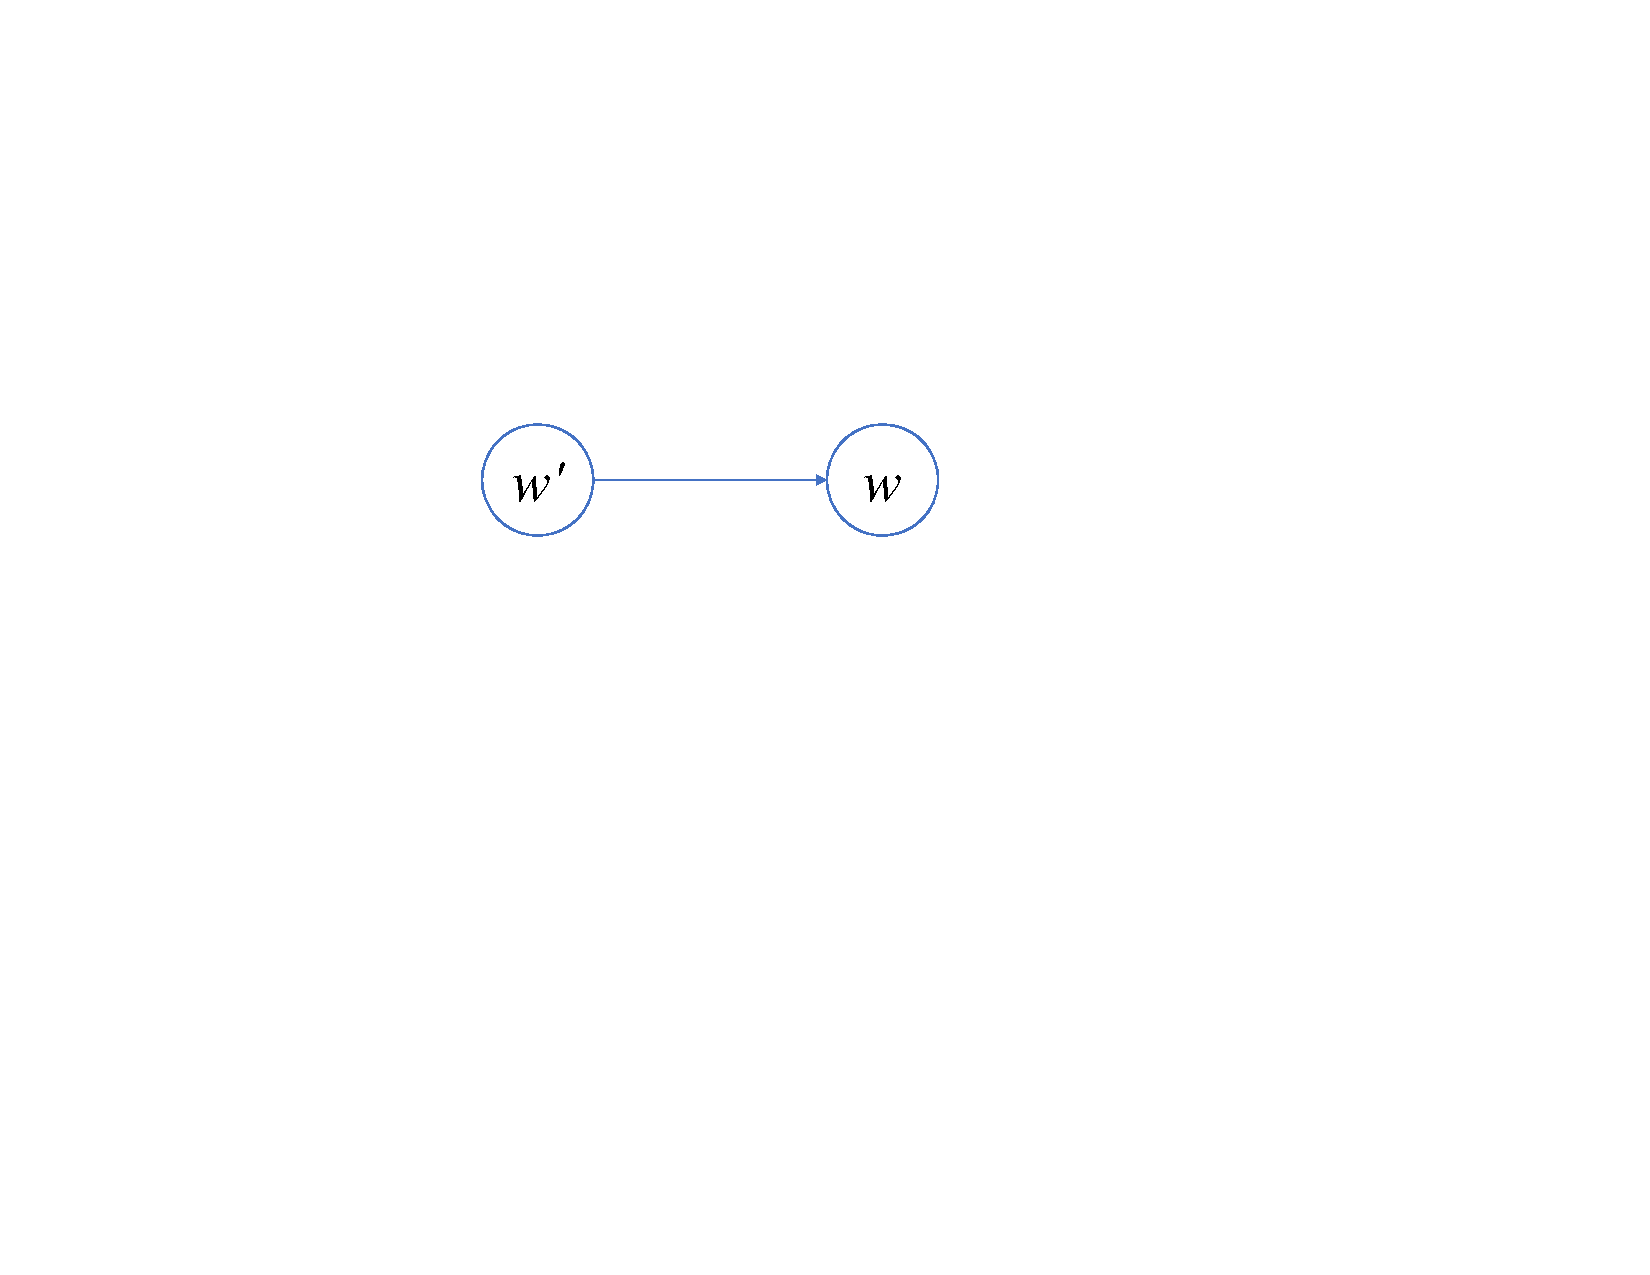
\includegraphics[width=0.14 \textwidth,]{./img/mc}}~
	\subcaptionbox{
		HMM
	}{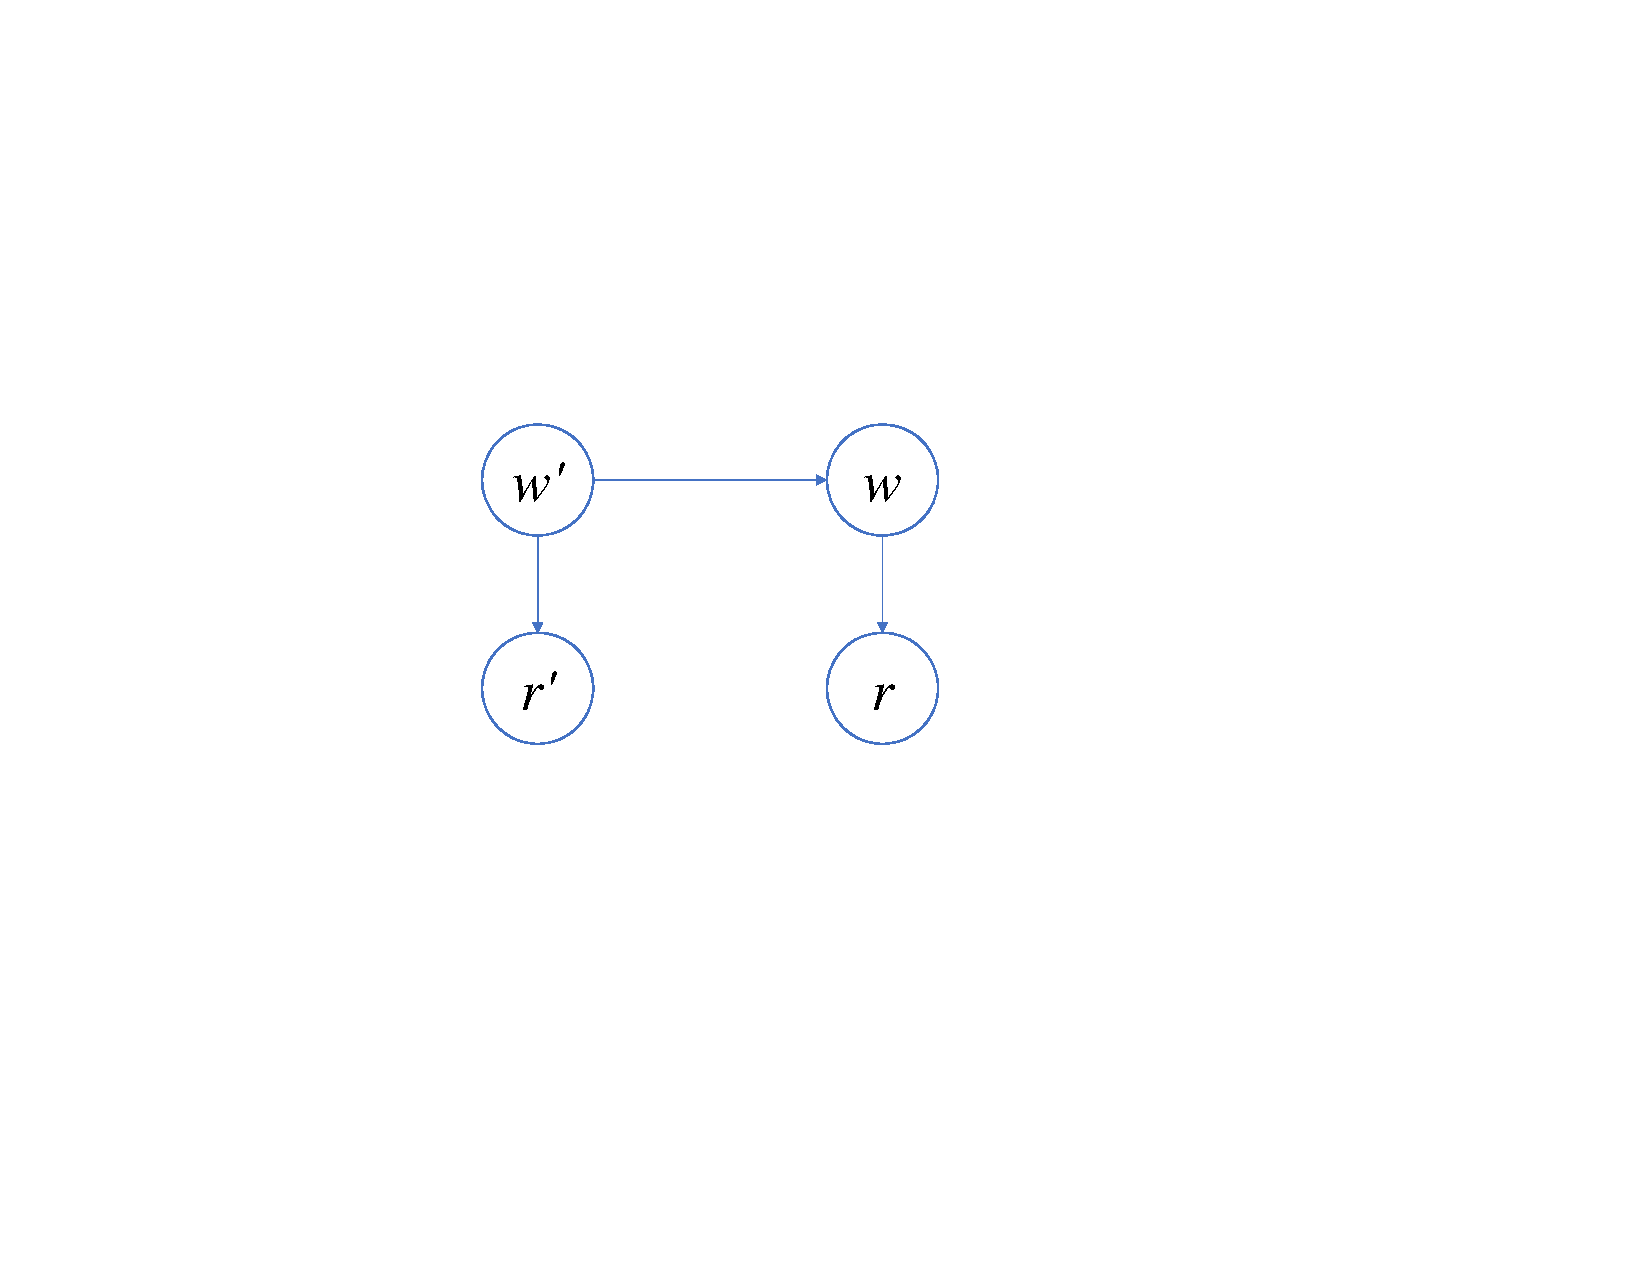
\includegraphics[width=0.14 \textwidth,]{./img/hmm}}~
	\subcaptionbox{
		HsMM
		\label{fig:hsmm2}
	}{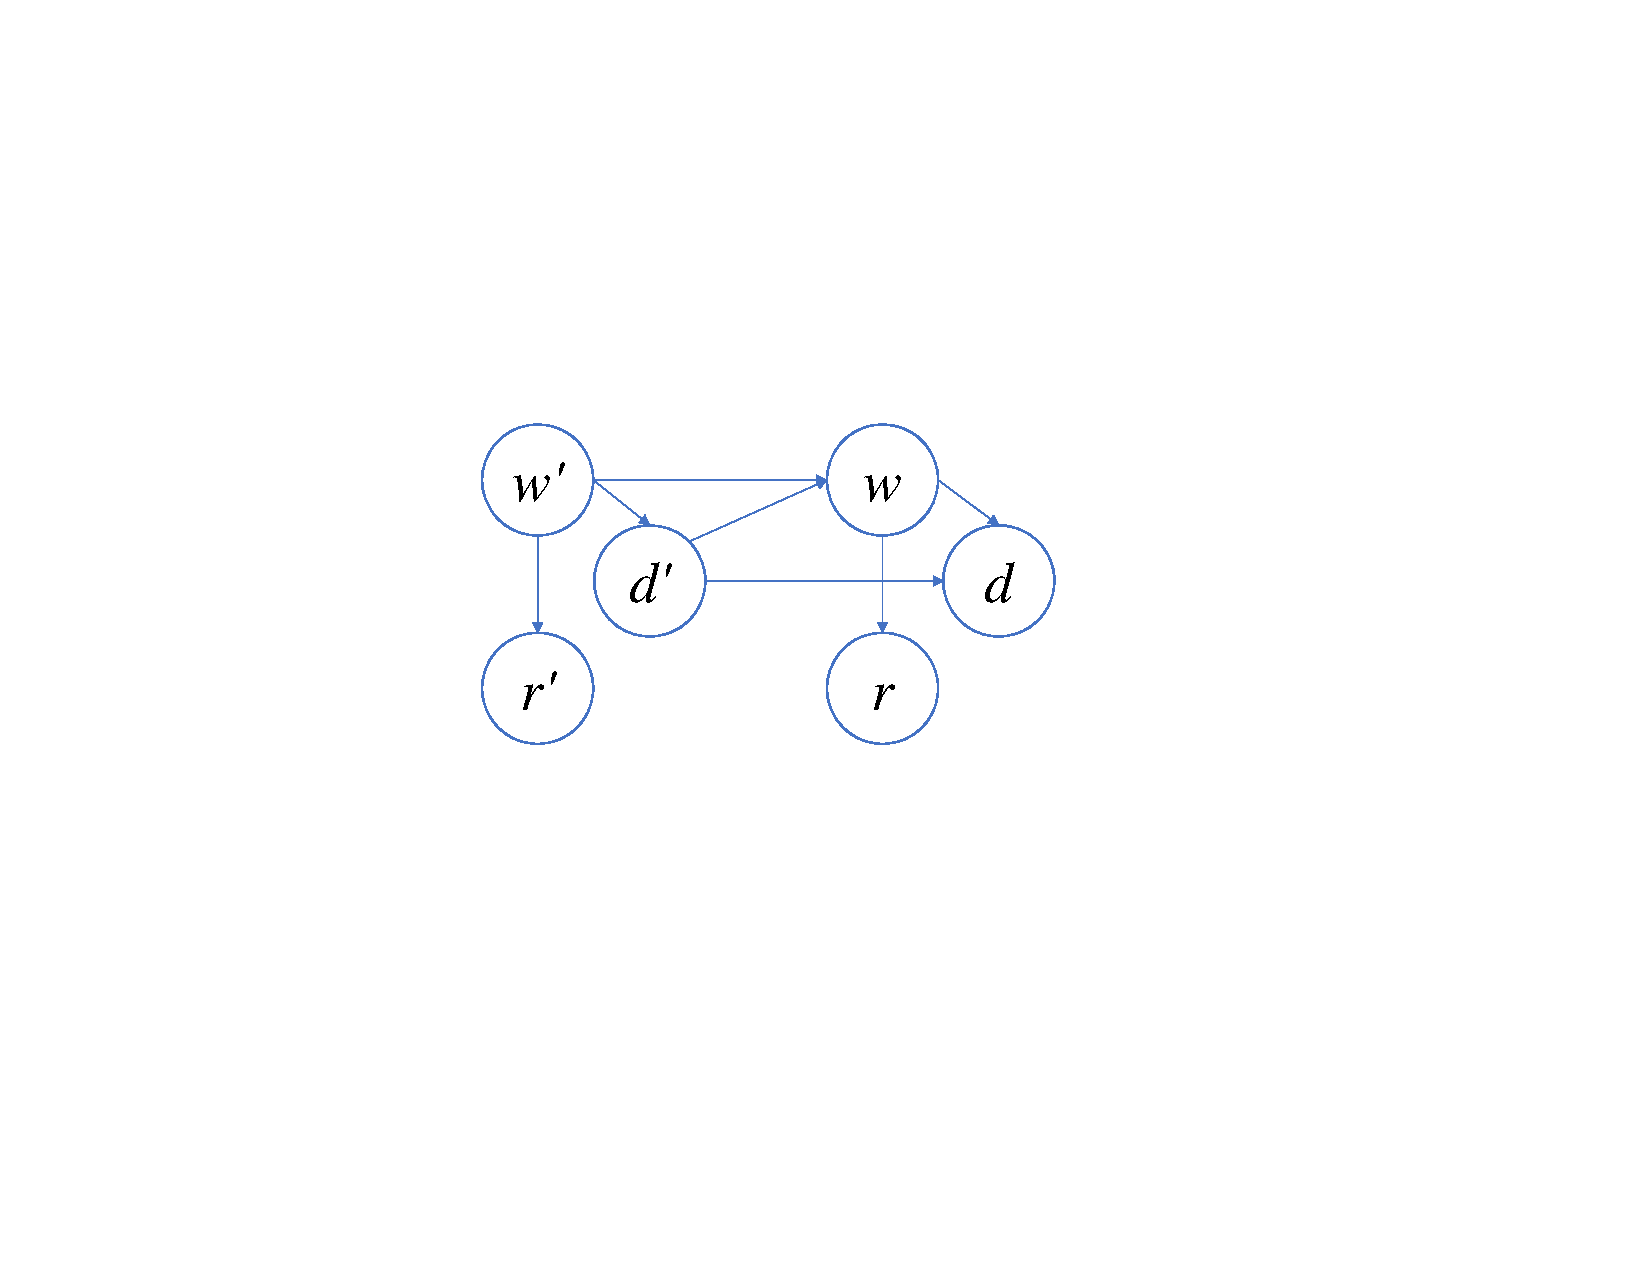
\includegraphics[width=0.17 \textwidth]{./img/hsmm2}}
	\caption{User's browsing models.}
	\label{fig:hsmm}
\end{figure}	
	
	
	
	\begin{equation}
	\label{eq:probs}
	\begin{alignedat}{3}
	\pr_u(w | w', d') &= 
	\begin{cases} 
	[\bP_u]_{w'w} & d' = 1  \\
	\delta(w, w') & d' > 1
	\end{cases} &,&
	\\ 
	\pr_u(d | w, d') &= 
	\begin{cases} 
	p_{w}(d) & d' = 1 \\
	\delta(d, d'-1) & d' > 1
	\end{cases} &,&
	\\   
	\pr_u(r|w) &= [\O_{u}]_{w, r}&,&	
	\end{alignedat} 
	\end{equation}
	
	The duration parameter can not be zero, when $d = 1$ the page's last request is submitted and the user moves to another page which resets the duration using $p_w(d)$. 
	The duration probability $p_w(d)$ determines the number of requests that the webpage $w$ will query and is independent of user $u$. 
	%	Also, the output probability $\o_{w}(r)$ only depends on the webpage $w$. 
	
	\begin{table}
		\centering
		\begin{tabular}{|c|l}
			\hline
			Symbol & Explanation \\ 
			\hline 
			%$U$ & Random variable for the active user \\ \hline
			$W$ & RV for the webpage \\ \hline
			$D$ & RV for the number of requests to be issued on a page \\ \hline
			$R$ & RV for the issued DNS request \\ \hline
			\hline 
			$m$ & Number of users \\ \hline
			$n$ & Total number of pages \\ \hline
			$q$ & Maximum number of requests per page \\ \hline 
			\hline 
			$\P_u \in \reals^{n \times n}$ & Webpage transition matrix of the user $u$ \\ \hline 
			$p_w(d), d \in [q]$ & Distribution of number of requests $d$ on the page $w$ \\ \hline 
			$\O_u \in \reals^{n \times n}$ & Output distribution matrix of the user $u$  \\ \hline
		\end{tabular}
		\caption{Summary of the model parameters and random variables (RV). For each random variable the corresponding small letter represents a realization. Note that $W$ and $D$ depend on the user but to avoid cluttering we omitted the index $u$.}
		\label{tab:params}
	\end{table}
	
	\subsection{Resolver's Sequence Interleaving Model}
	\label{subsec:interle}
	As mentioned in Section \ref{subsec:nature}, we have access only to the resolver data queue where users enqueued their domain name requests. 
	Here we assume that there is a Markov chain governing the ``turn'' of users. 
	Let's assume that we have $m$ users.
	We name the transition matrix of the user's Markov chain as $\A = [\alpha_{ij}] \in \reals^{m \times m}$.
	Therefore the probability of user $j$ generating the $t$-th request given the current user as $i$ is $\pr(U(t)=j|U(t-1)=i) = \alpha_{ij}$.
	The random variable $U(t) \in [m]$ represent the active user that has generated the $t$th request of the resolver queue. 
	
	%	We define the interleaving process as follows.
	%	To generate the $t$-th request, first we should determine the active user and then a user $i$ is selected to generate the $t$th request in the resolver queue with probability $\alpha_i$. 
	%	More formally, the random variable $U(t)$ represents the user that generates the query at $t$th place of the resolver's queue. 
	A simplification of the transition matrix that has been use in literature is $\forall i, j: \pr(U(t) = i|U(t-1) = j) = \alpha_i$, where the whole dynamic of the system can be represented by a single users \emph{shares vector} $\aalpha$ instead of the \emph{users transition matrix} $\A$.
	
	To distinguish each user's corresponding HsMM random variable in the interleaving process we use both user index and time index. For example, $W_{k}(t)$ is the user $k$'s current webpage. 
	Note that here the time is different from the real world time and HsMM duration that discussed in Section \ref{subsec:user}. 
	Time here is just an index into the resolver's sequence of queries.
	For example, $W_{k}(t)$ shows the webpage of user $k$ when the $t$th request was submitted to the resolver. 
	Note that, the $t$th request may have been generated by any of the users not only $k$. 
	
	To elaborate the interleaving process, we describe it as an Augmented Hidden Markov Model (AHMM), where the hidden states are augmented state, i.e., combination of variables \cite{minot2014separation}. 
	To make the equations more readable, we lump together the variables corresponding to each user and make the following lumped variable $L_k(t) = (W_{k}(t), D_{k}(t))$ and the hidden state of the HMM becomes $H(t) = (L_1(t), \dots, L_m(t), U(t))$ which is a $2m +1$ dimensional vector.
	Fig \ref{fig:rq} illustrates the interleaving process that leads to sequence generation.
	To avoid cluttering in the following we assume $u(t-1) = u'$ and $u(t) = u$ which means that users $u'$ and $u$ are active at time steps $t-1$ and $t$ respectively. 
	\begin{figure}
		\centering
		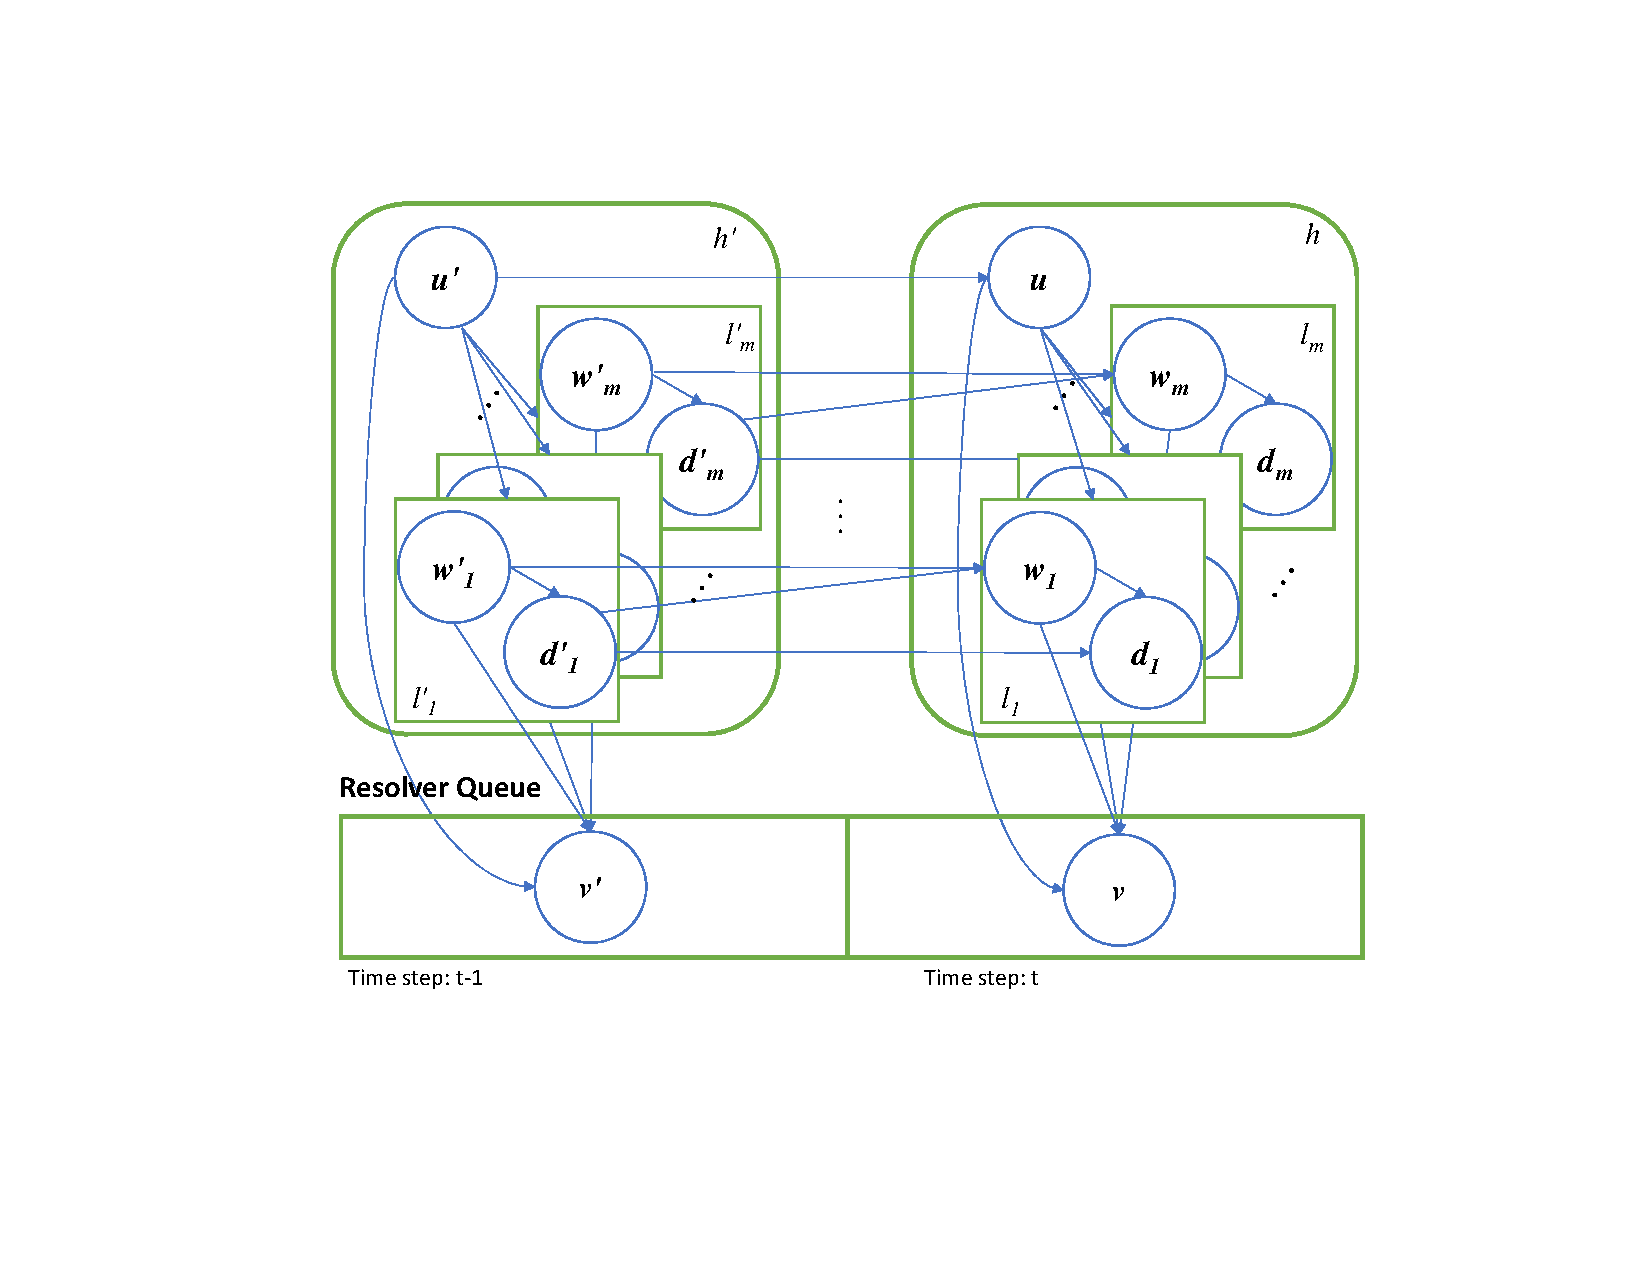
\includegraphics[width=.45\textwidth]{./img/hsmm-q2}
		\caption{Illustration of the interleaving process.}
		\label{fig:rq}
	\end{figure} 
	
	%Let's name the $t$th request in the queue as  at the time step $t$.  
	At the time step $t$, user $u(t) = u \in [m]$ generates the request $v(t)$ which is the observed (visible) variable of the HMM.
	The request $v(t)$ is determined by the next request of the user in its HsMM model, i.e., $r_{u}(t)$.	
	Therefore, the emission probability of the AHMM is:
	{\small
	\be 
	\nr 
	\pr(V(t) = v(t) | H(t) = h(t)) = \pr_{u}(r_{u}(t) | w_{u}(t)) = \O_{u}(w_{u}(t), r_{u}(t)).
	\ee 
	}
	%	Note that the emission probability is still only a function of the page $w$ but to keep track of each users current page we introduced $u$ as an index $w_u$, meaning that we are looking at the page that is browsed by user $u$. 
	%	We call the emission probability matrix that is built from $\o$s (in a way that is describe below) as $\E$.
	%	From now on, we omit the time index of $u(t)$ to avoid cluttering.
	Now we derive the entries of the transition probability matrix of the AHMM:
	\be 
	\pr(H(t) | H(t-1)) = \alpha_{u'u} \prod_{k=1}^{m} \pr(l_k(t) | l_k(t-1), u),
	\ee 
	%	where 
	%	\be
	%	\pr(l_k(t) | l_k(t-1), U(t) = u) = 
	%	\begin{cases}
	%		\pr_u(x | x', s') \pr_u(s | x, s') & u = k\\
	%		\delta(x, x')\delta(y, y')\delta(s, s')\delta(r, r') & u \neq k
	%	\end{cases}
	%	\ee 
	%	where $U(t) = j$. 
	In the case of $k \neq u$ the user $k$ is not active, i.e., stalled. 
	Substituting the probability distributions from \eqref{eq:probs}, we get: 
	\be
	\pr(l_k(t) | l_k(t-1), u) = 
	\begin{cases}
		k \neq u & \delta(w, w')\delta(d, d') \\
		k = u & 
		\begin{cases}
			d = 0 & p_w(d) [\P_u]_{w'w} \\
			d > 0 & \delta(d, d-1)
		\end{cases}  		
	\end{cases}
	\ee 
	
	\begin{table}
		\centering
		\begin{tabular}{|c|l|}
			\hline
			Symbol & Explanation \\ 
			\hline 
			$L$ & The lumped random variable $L = (W, D)$. \\ \hline
			$H$ & The hyper-hidden state of the HMM $H = (L_1, \dots, L_m, U)$.\\ \hline
			$V$ & The visible state of the HMM which is the requested DN. \\ \hline 
		\end{tabular}
		\caption{Summary of the augmented variables. For each random variable the corresponding small letter represents a realization.}
	\end{table}
	
	\section{Deinterleaving Methods}
	In the deinterleaving problem, given $\{v(t)\}_{t=1}^T$ we are
        interested in inferring $\{u(t)\}_{t=1}^T$.  In other words,
        we want to find the users who initiated each request from the
        sequence generated by the interleaving process described in
        Section \ref{subsec:interle}.
	
	We present two candidate approaches for inference.  One is
        based on reducing the interleaving process to an AHMM as
        discussed in Section \ref{subsec:interle}.  This approach has
        been used for deinterleaving of Markov chains with small
        number of chains (users) and state space
        \cite{minot2014separation}.  Next, we propose to deinterleave
        using an RNN and an LSTM model which have recently been shown to 
        perform well in many time-series analysis tasks\cite{chung2014empirical,Hochreiter}.
	
	\subsection{Inference on Augmented HMM}
        We can model the whole interleaving process as an AHMM
        and use learning techniques (like
        EM) to learn its parameters and use Viterbi inference to
        determine the most probable hidden (augmented) states $h(t)$
        from which we can extract the most probable user $u(t)$.  The
        main difficulty of applying this framework is that the state
        space of hidden variable, Figure \ref{fig:hsmm}, is very
        large.  More specifically, there are $m (nq)^m$ possible
        states of $h$ and as we increase number of webpages $n$ or
        users $m$ the state space grows exponentially.  The huge state
        space, makes the inference and learning very hard and as we
        show in Section \ref{subsec:viterbi} for synthetic
        experiments, even when the model parameters are known,
        deinterleaving performs (using Viterbi coding) poorly.
	
	\subsection{Inference using an RNN}
        RNNs \cite{lecun2015deep} are popular for modeling time
        series data. Given the input $v_t$ and hidden state $h_{t-1}$,
        the RNN computes the next hidden state representation $h_t$
        and output $u_t$ using the following recurrent relationships
	\begin{align}
	\label{eq:rnn}
	h_{t} &= f(W_v v_{t} + W_h h_{t - 1} + b)\\
	u_t &= W_u h_t
	\end{align}
	%
	where $W_v$, $W_h$, $W_v$ and $b$ are the network parameters, and $f()$ is some non-linear function. 
        An example of $f$ could be a sigmoid $f(z) = \sigma(z) = 1/(1+\exp(-z))$ or rectified linear unit $f(z) = \max(0,z)$. 
	
	
	For our specific problem of deinterleaving, an RNN can 
        by posed as a multi-class classification problem, where
        the input is the observed webpage and the output will be the
        identified user who requested that webpage. Specifically, each
        data instantiation consists of a sequence of user-request
        pairs, i.e., $(u(t), v(t))$.  This represents who was the user
        at a given time $t$ and what request was produced by that
        user. Both the user and the request are represented by an
        integer. The RNN is unrolled for the entire length of one
        sequence. The users and request integers are converted to
        one-hot encoding to enable learning. Thus if there are $b$
        possible web pages, the requests become $b$-dimensional
        vectors and for $m$ users, it becomes an $m$-dimensional
        vector. The request vectors are fed as input to the RNN model,
        while the output is the corresponding user at each
        time-step. The RNN’s $m$-dimensional output is passed through
        a softmax layer to convert it into probabilities and the user
        with higher probability is compared against the ground
        truth. Performance is measured in terms of accurately
        identifying the user at each instant.
	
	A common approach to solving the optimization problem is to
        randomly initialize network parameters $W_v, W_h, W_u$ and
        apply stochastic gradient descent (SGD) (for RNNs, it is also
        referred to as a Backpropagation-through-time (BPTT)
        algorithm). In particular, we use a variation of the standard
        SGD called Adam \cite{kingma2014adam}, which allows for
        adaptive learning rates using the past gradients, similar to
        using momentum. This results in faster convergence compared to
        other adaptive algorithms.
	
	
	
	
		\section{Experiment}

%	We have used an LSTM based model for user identification. Each data instantiation consists of a sequence of user-request pairs. This represents who was the user at a given time instant and what request was produced by that user. Both the user and the request are represented by an integer. The LSTM is unrolled for the entire length of one sequence. The users and request integers are converted to one-hot encoding to enable learning. Thus if there are $b$ possible web pages, the requests become $b$-dimensional vectors and for m users, it becomes a m-dimensional vector. The request vectors are fed as input to the LSTM model, while the output is the corresponding user. The LSTM’s m-dimensional output is passed through a softmax layer and the user with higher probability is compared against the ground truth. Performance is measured in terms of accurately identifying the user at each instant.
	
	
	
	
	We start with a synthetic toy example and compare our LSTM inference algorithm with Viterbi as the baseline and then move to larger experiments.
	In all experiments, LSTM is trained, validated and tested with sequences of size 6, 3, 1 thousands requests, respectively. 
	
%	For the synthetic experiments, we first compare the performances of the Viterbi-based and RNN-based methods in a toy example and then move to examples with larger state space for detail examination of the RNN-based methods. 
	%	The main inference algorithm that we are interested in is the Viterbi algorithm to infer the hidden states and extract the corresponding users. 
	%	Knowing the model parameter, we check the Viterbi's performance. 
	%	In the next step, we move to the parameter learning through the Baum–Welch algorithm, which in turn requires Forward-Backward algorithm. 
	%	Finally using the learned parameter we check the performance of the Viterbi. 
	
	%	\subsection{Sample Sequence Generation}
	%	There are two ways that we can generate the synthetic data. 
	%	The first one is in the time domain where we have a group of users independently browse pages and generate DNS requests and submit it to the resolver. 
	%	At the end, we take the queue of the resolver as the input for our algorithm. 
	%	The second method is to build the exact generative model of Section \ref{sec:gen}, i.e., the interleaving HsMMs, and from that generate a sequence of domain queries.
	%	In the following, we generate data using both methods. 
	%	
	%%	\subsubsection{Simulation in the Time Domain}
	%%	The detail of implementation is in the dgen.py file. 
	%	\subsubsection{Simulation of the HMM Model}
	%	First we generate a lookup table that maps each hyper-state ID to a corresponding \emph{state code}.
	%	We use the following string code for each hyper-state of the HMM:
	%	\be
	%	\underbrace{\Box\dots\Box}_{\substack{1\dots c \\ u}}, \underbrace{\Box\dots\Box}_{\substack{1\dots c \\ w_0}}, \underbrace{\Box\dots\Box}_{\substack{1\dots c \\ d_0}},\dots,
	%	\underbrace{\Box\dots\Box}_{\substack{1\dots c \\ w_{m-1}}},
	%	\underbrace{\Box\dots\Box}_{\substack{1\dots c \\ d_{m-1}}},		 
	%	\ee 
	%	$c=\log_{10}(\max(m,n,q))$ is the \texttt{CODE\_SIZE} and each number is zero-filled to fill the whole sub-string of size $c$. 
	%	The active user of the state is $u$, $w_i$ and $d_i$ are the current page and remaining number of requests in the page of the $i$th user.
	%	
	%	For example, for the code size of two, ``$01,00,02,10,05$'' is the state in which user 1 is active, and on page 10 and there are 5 more requests to be submitted from the page 10. User 0 should wait on page 0 to submit its 2 remaining requests. 	
	%	
	%	Number of states depends on number of users, pages, and requests per page. 
	%	It can be computed as $s = m n^m q^m$ where $m$ is the number of users, $n$ is the number of pages and $q$ is the maximum number of queries/requests possible in each page (duration in the HsMM).  
	
	\subsection{Viterbi vs. RNN}
	\label{subsec:viterbi}
	Here we generate synthetic resolver queue using the most complicated user model, i.e., HsMM of Figure \ref{fig:hsmm2} and report the Viterbi and LSTM methods performance. 
	To reduce the computational burden for the Viterbi algorithm, we restrict ourselves to 2 pages, 2 users, and 2 possible requests per page. 
	To make the setup even simpler, user $i$ browse only page $i$ and page $i$ picks from two possible requests at random using Beta(3+$\epsilon$,1+$\delta$) where $\epsilon$ and $\delta$ are independent and uniform over $[0,1]$.
	Viterbi is tested on the same sequences of size thousand. 
	Results are averaged over 5 realizations of the synthetic data. 
	%In the MC and HMM user models, this results in an AHMM with 8 hidden states and 2 observation. 
	With this setup the size of the hidden state space of the AHMM built from the HsMM user model is 32 and the number of observations is 2. 
	The users shares vector is $\aalpha = (.4, .6)$.
	
	Table \ref{tab:viterbi} summarizes the result:
	\begin{table}
		\scriptsize  
		\centering
		\begin{tabular}{|c|c|c|}
			\hline
			{\bf Method} & {\bf Viterbi} & {\bf LSTM} \\ 
			\hline  			
			Mean Accuracy	& 0.51	&  0.92  \\ \hline 
			Std of Accuracy	& 0.02		&  .17  \\ \hline 
		\end{tabular}
		\caption{Comparing accuracy of Viterbi coding and LSTM methods for the toy example. Results are averaged over 5 realization of the synthetic data.}
		\label{tab:viterbi}
	\end{table}
	Interestingly, LSTM outperform Viterbi with a large margin. 
	Note that we perform Viterbi assuming that HMM parameters are given, and even with this setup Viterbi performs poorly. 
	
	\subsection{Synthetic Experiment}
	\label{subsec:synthetic}
%	{\color{red} All of the results after this part should be re-done using the TensorFlow code.}
	Owing to the poor performance of AHMM approach from now on we focus on LSTM method of Section ?.
	We report the results of seven synthetic experiments only for LSTM. %: toy example, scaling users, and scaling pages.
	%In all set of experiments, we generate 100 different sequence of length 1000 according to the request generation and interleaving process of Sections ? and ?.
	%The entire data for each instantiation, (100 different sequences) is divided into training, validation and test sets in the ratio 0.6, 0.2 and 0.2 respectively. 
	%The model parameters that perform the best on the validation set are saved and using these parameters, the results are reported on the test set. 
	%The RNN is trained using the Adam optimizer.
	%\subsubsection{Different Browsing Scenarios}
	%In this toy example 
	We test the results for 7 different scenarios, in all of them we want to deinterleave a sequence generated by two users but the parameters in each experiment is set up differently.
	Table \ref{tab:toy} specifies the shared parameter setup. % for the toy example.
	Specific user transition and emission matrices are set for different scenarios which are explained in Section \ref{subsub:sparsity}.
	Note that in our experiments we report results on two set of synthetic data set, where in one we have a users shares vector $\aalpha$ determining the share of each user from the queue's requests.
	In the other more general data generating scheme, we assume that the users transition matrix $\A$ governs the turn in request submission.
	Different distributions for $\aalpha$ and $\A$ are discussed in Section \ref{subsub:dist}.
	
	\begin{table}
		\centering
		\begin{tabular}{|c|l|}
			\hline
			Parameter & Value \\ 
			\hline  
			$m$ & 2 users \\ \hline
			$n$ & 20 pages \\ \hline
			$q$ & Maximum of 5 request per page\\ \hline 
			\hline 
			$\aalpha$ & $[0.4, 0.6]$ \\ \hline 
			$\A$ & Diagonal dominated row stochastic random matrix$^*$. \\ \hline 
			$\P_u$ & A random $20 \times 20$ matrix$^*$ \\ \hline 			
			$p_w(d)$ & $\text{Uniform}(1,5)$ \\ \hline 
			$\O_u$ & A random $20 \times 20$ matrix$^*$ \\ \hline 
		\end{tabular}
		\caption{Summary of the experimental setup for the synthetic experiment \ref{subsec:synthetic}. $^*$More on the random matrix generation in the text.}
		\label{tab:toy}
	\end{table}
	
	{\bf Sparsity Patterns of Matrices:}
	\label{subsub:sparsity}
	For each user $u$ we have two matrices $\P_u$ and $\O_u$ which are randomly generated. 
	The generation process assumes that each row of both matrices is sparse, which is a reasonable assumption. 
	Each user view and surf a limited number of pages and on each page the possible requests are from a small subset of the all available pages. 
	The supports of $\P_i$s and $\O_i$s can overlap or be disjoint and this combination generates the different setups of our experiments.  
	%	We hypothesize if users surf disjoint subset of webpages deinterleaving would be easier. 
	After selecting a support we generate a discrete distribution over that support, which will be discussed in Section \ref{subsub:dist}.
	
	In the following the outer-list determines the different strategies for generating $\P_u$s and the inner-list elaborates the method of building $\O_u$s. 
	Each row of $\O_u$s has $a$ non-zero elements (randomly selected) and the distribution is uniform.
	When call $\O_1 \neq \O_2$ and $\O_1 = \O_2$ schemes, personalized and shared outputs respectively.
	
	\begin{itemize}
		\item {\bf Disjoint webpage surfing:}  In this scenario, users surf disjoint parts of the web, say user 1 surf inside a group of first $a$ pages and user 2 surf the remaining $n - a$ pages, Fig \ref{fig:dsurf}.
		%		So $\P_u$s are block matrices similar to Fig ?.
		\begin{itemize}
			\item[] {\bf Case 1)} \emph{Disjoint personalized outputs - same grouping as webpages:} $\O_u$ and $\P_u$ have similar sparsity patterns, Fig \ref{fig:case1}. 
			\item[] {\bf Case 2)} \emph{Disjoint personalized outputs:} $\O_u$ and $\P_u$ do not have similar sparsity patterns, but support of $\O_1$ and $\O_2$ are disjoint, Fig \ref{fig:case2}. 
			\item[] {\bf Case 3)} \emph{Shared output:} $\O_1 = \O_2 = \O \in \reals^{n \times n}$ , Fig \ref{fig:case3}.
		\end{itemize}
		\item {\bf Overlapped webpage surfing with fixed block size: }
		Each user selects its surfing support of size $a$ at random. 
		Supports may overlap, Fig \ref{fig:osurf}. 
		\begin{enumerate}
			\item[] {\bf Case 4)} \emph{Personalized outputs:} $\O_1 \neq \O_2 \in \reals^{n \times n}$, Fig \ref{fig:case4}. 
			\item[] {\bf Case 5)} \emph{Shared output:} $\O_1 = \O_2 = \O \in \reals^{n \times n}$ , Fig \ref{fig:case5}.
		\end{enumerate}
		\item {\bf Overlapped webpage surfing with variable block size and interaction between blocks: }
		Each user selects $s = \text{Uniform}(1, a)$ pages at random as its main support (higher probability of surfing in these $s$ pages), and $a-s$ pages again at random as its auxiliary support (pages that user seldom visits), Fig \ref{fig:osurfau}.
		\begin{enumerate}
			\item[] {\bf Case 6)} \emph{Personalized outputs:} $\O_1 \neq \O_2 \in \reals^{n \times n}$, Fig \ref{fig:case6}. 
			\item[] {\bf Case 7)} \emph{Shared output:} $\O_1 = \O_2 = \O \in \reals^{n \times n}$ , Fig \ref{fig:case7}.
		\end{enumerate}
	\end{itemize}
	
	\begin{figure}
		\centering
		\begin{subfigure}[b]{0.15\textwidth}
			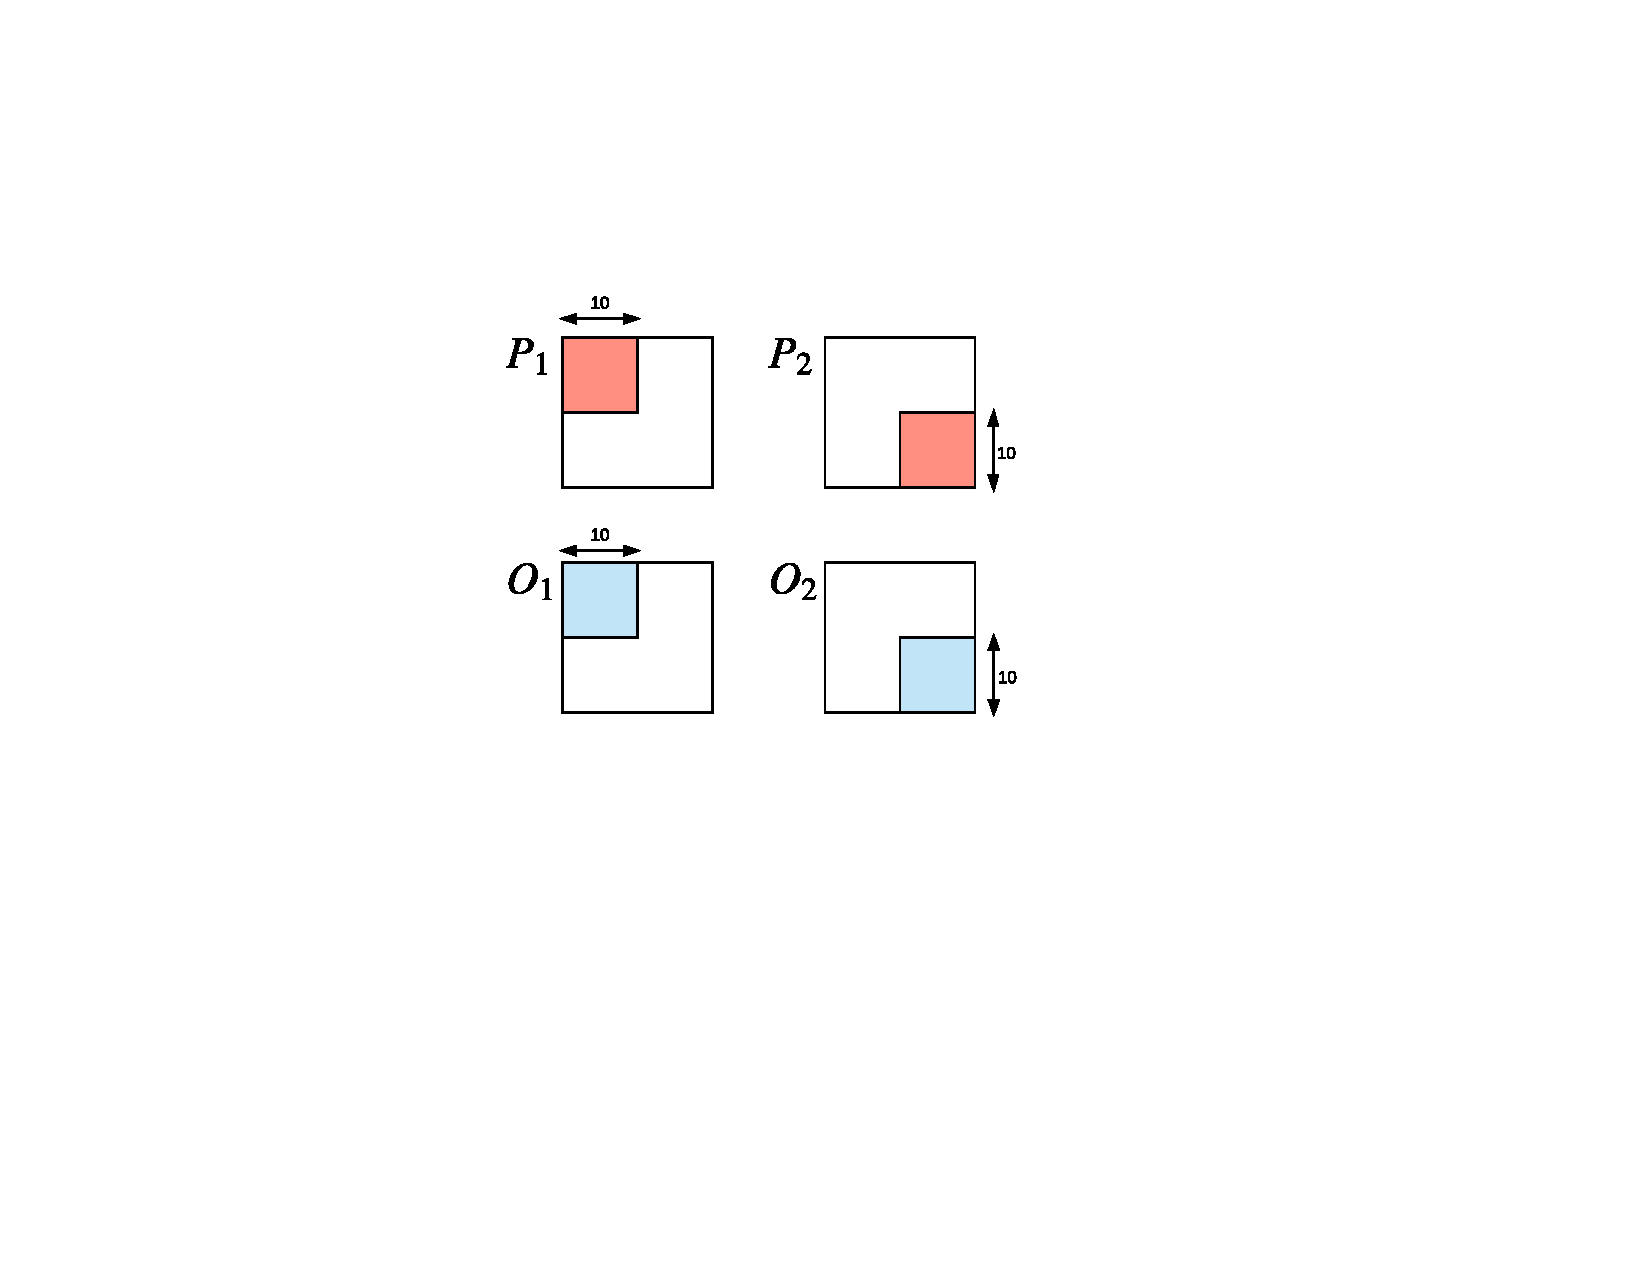
\includegraphics[width=\textwidth]{./img/case1-2}
			\caption{Case 1}
			\label{fig:case1}
		\end{subfigure}
		~ %add desired spacing between images, e. g. ~, \quad, \qquad, \hfill etc. 
		%(or a blank line to force the subFig onto a new line)
		\begin{subfigure}[b]{0.15\textwidth}
			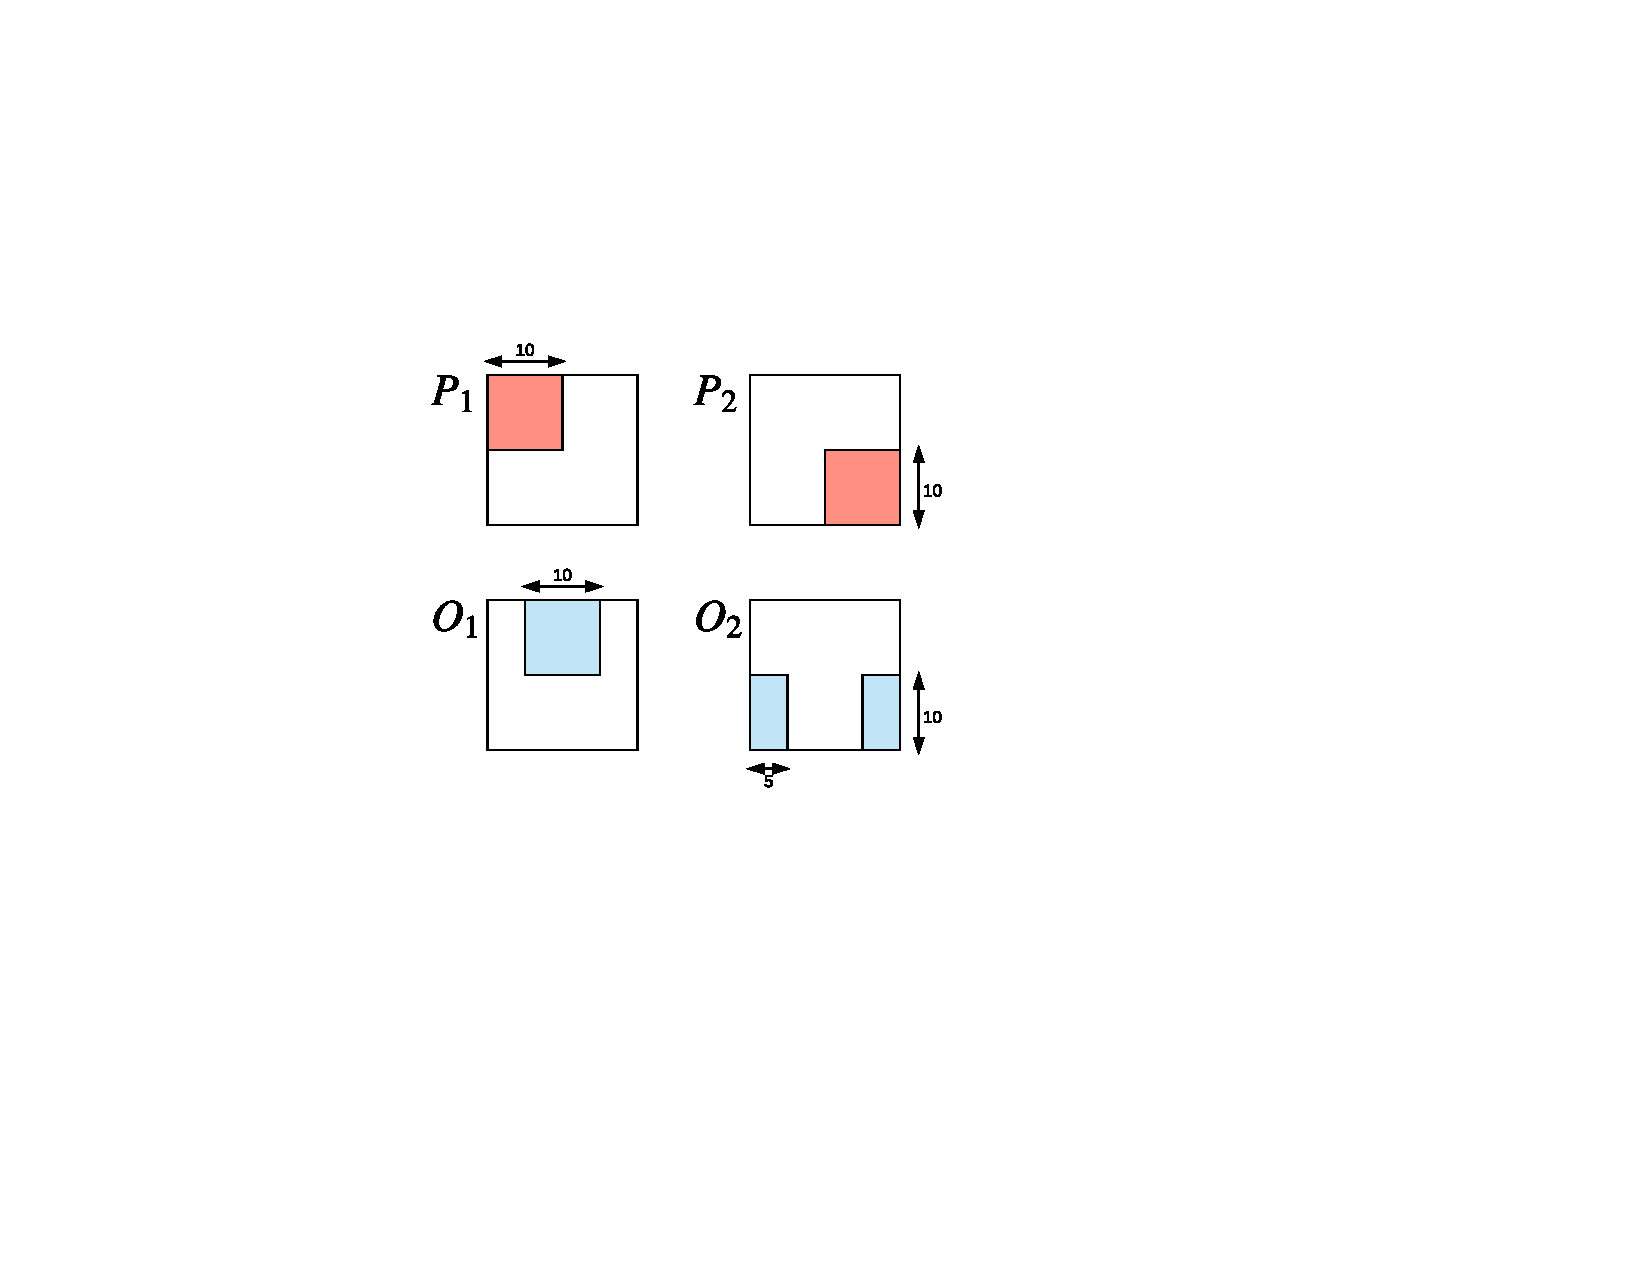
\includegraphics[width=\textwidth]{./img/case2-2}
			\caption{Case 2}
			\label{fig:case2}
		\end{subfigure}
		~ %add desired spacing between images, e. g. ~, \quad, \qquad, \hfill etc. 
		%(or a blank line to force the subFig onto a new line)
		\begin{subfigure}[b]{0.15\textwidth}
			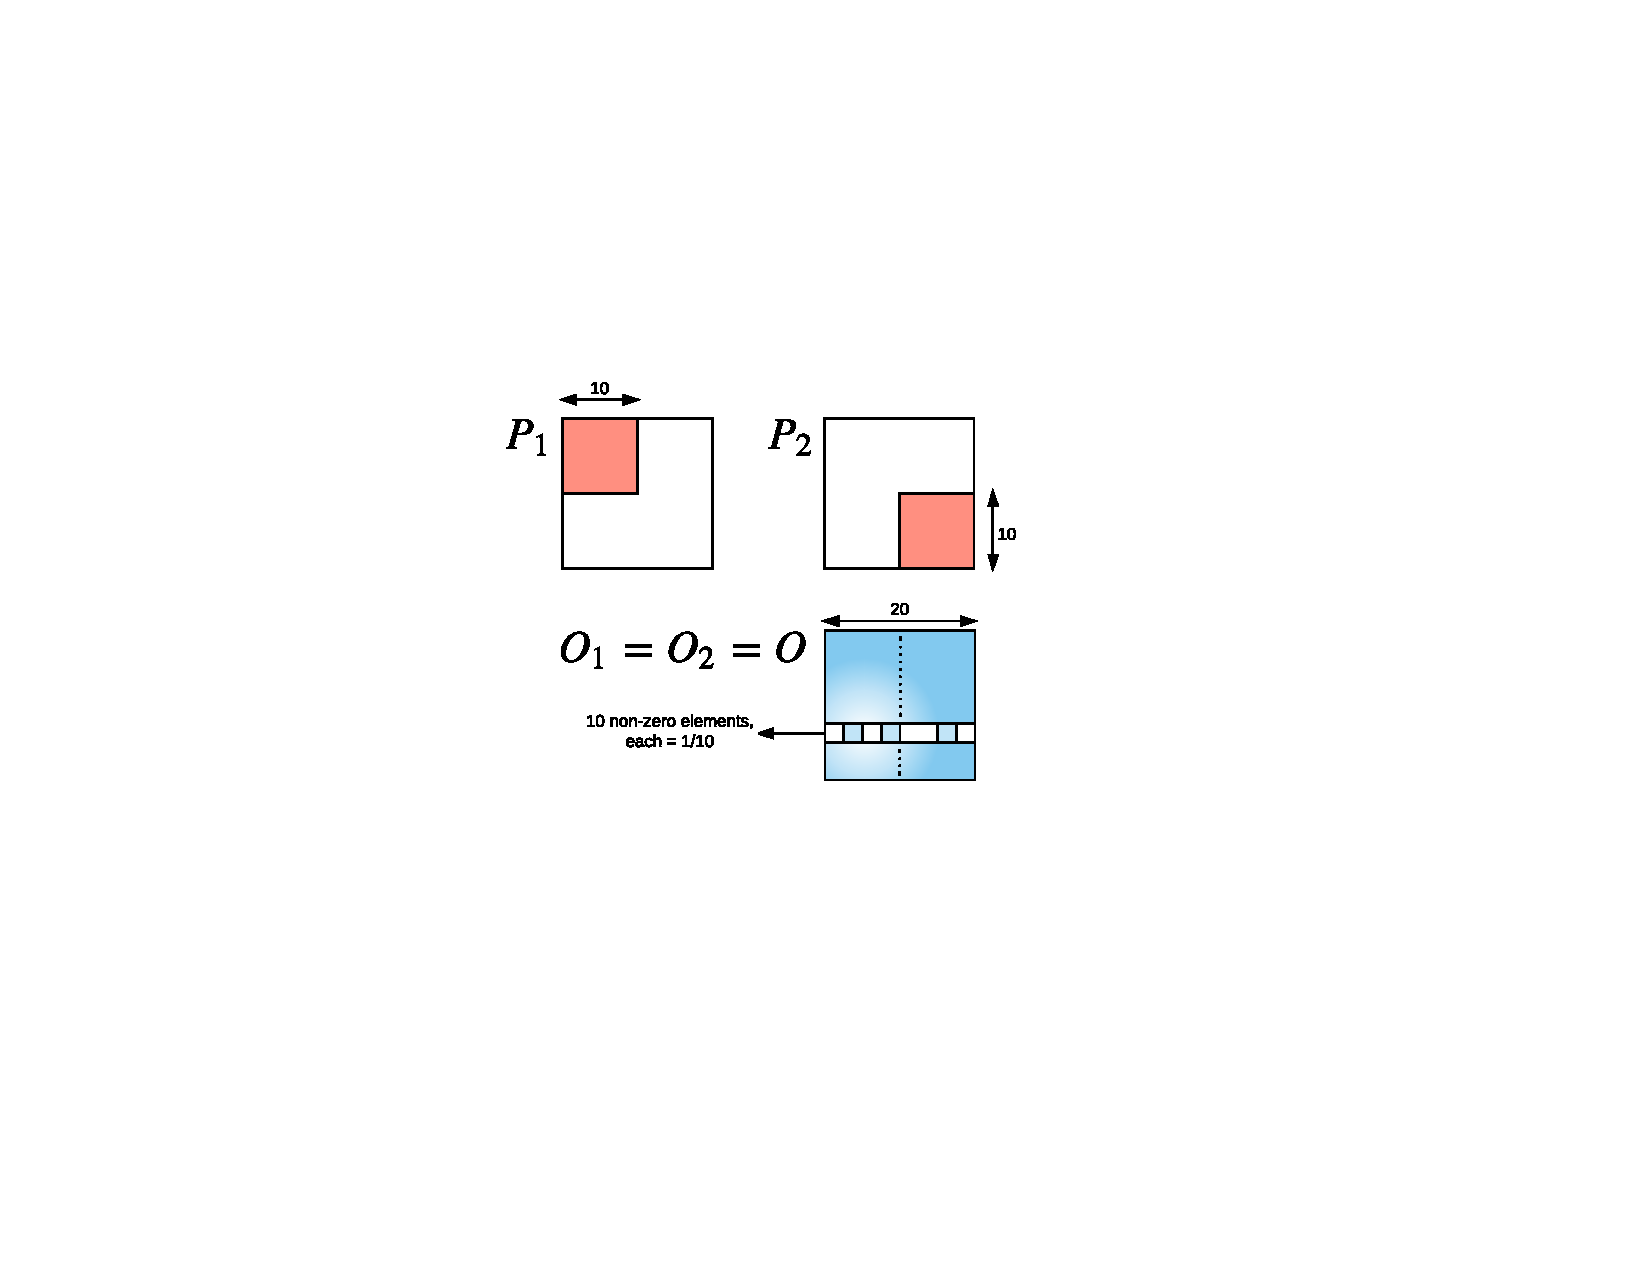
\includegraphics[width=\textwidth]{./img/case3-2}
			\caption{Case 3}
			\label{fig:case3}
		\end{subfigure}
		\caption{Illustration of the disjoint surfing categories for $a = 10$ and $b = 20$.}\label{fig:dsurf}
	\end{figure}
	
	
	\begin{figure}
		\centering
		\begin{subfigure}[b]{0.22\textwidth}
			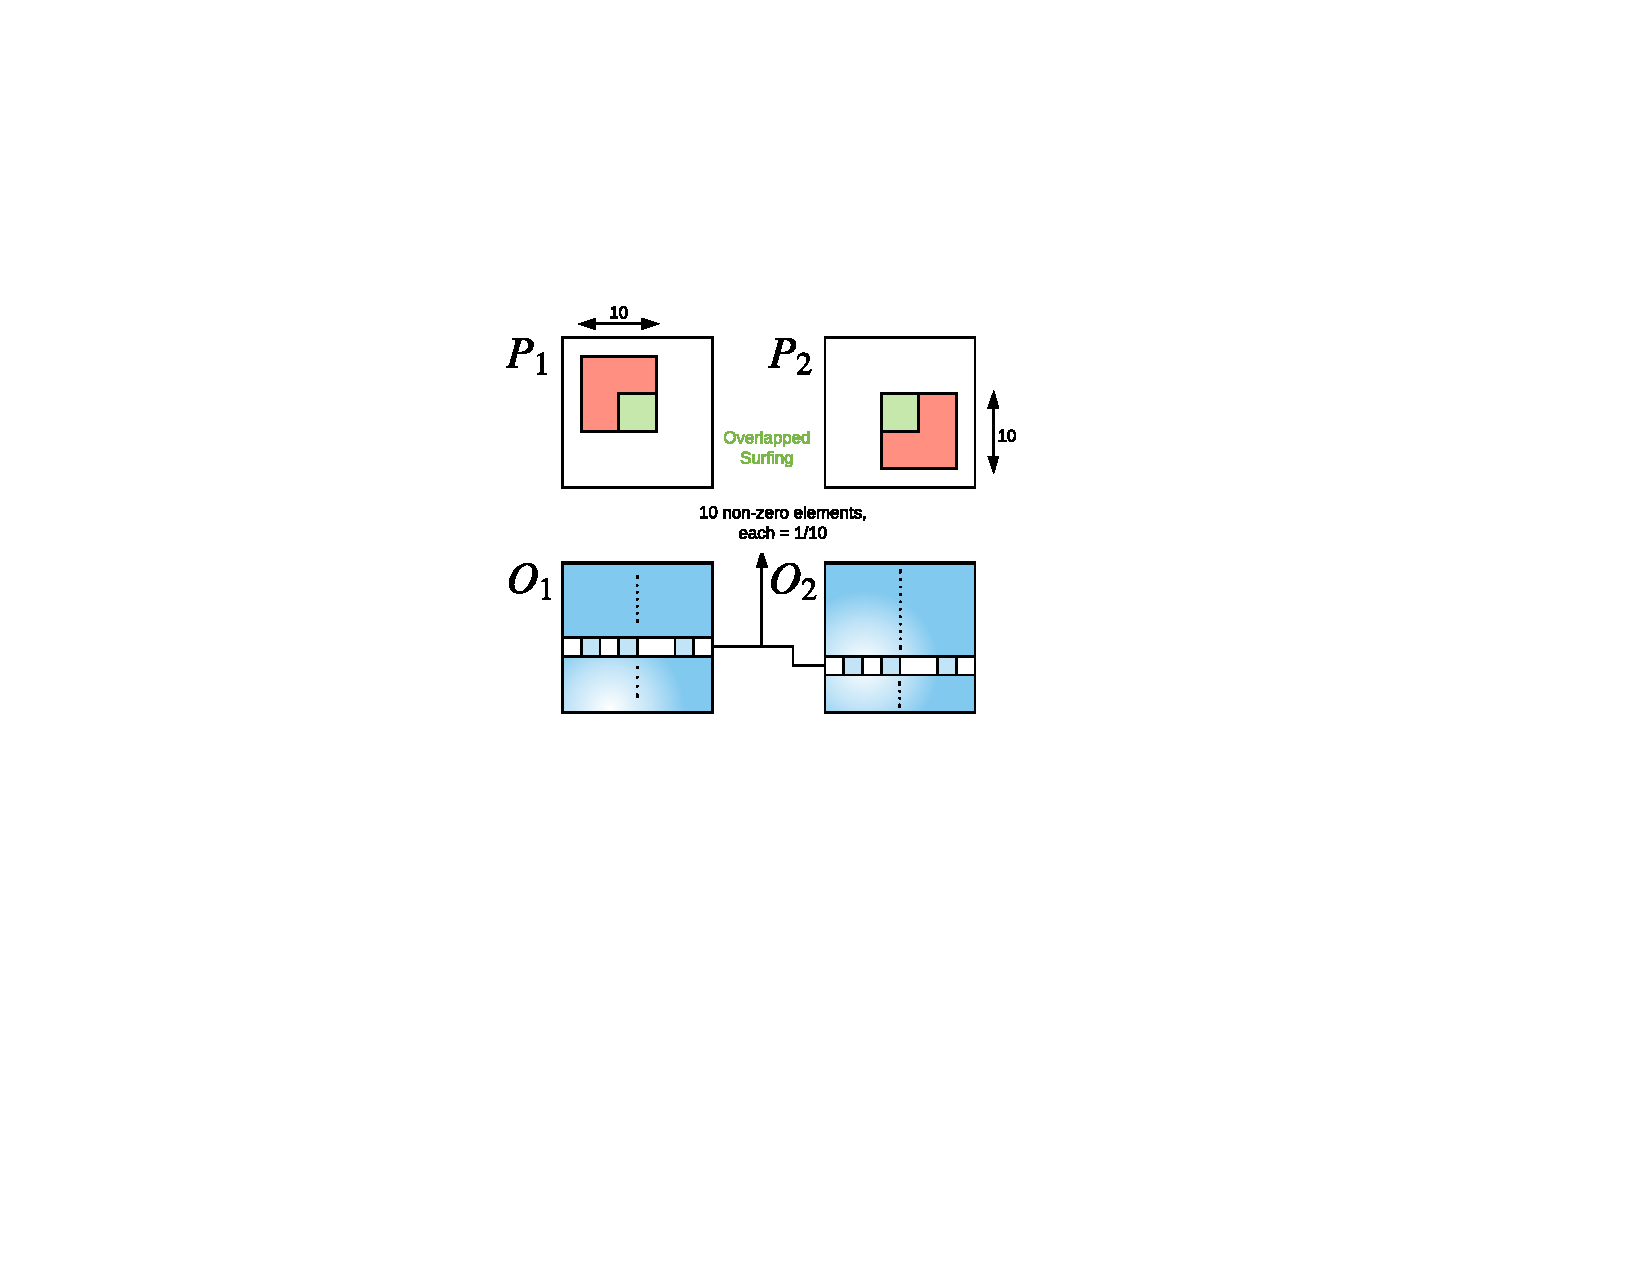
\includegraphics[width=\textwidth]{./img/case4-2}
			\caption{Case 4}
			\label{fig:case4}
		\end{subfigure}
		~ %add desired spacing between images, e. g. ~, \quad, \qquad, \hfill etc. 
		%(or a blank line to force the subFig onto a new line)
		\begin{subfigure}[b]{0.22\textwidth}
			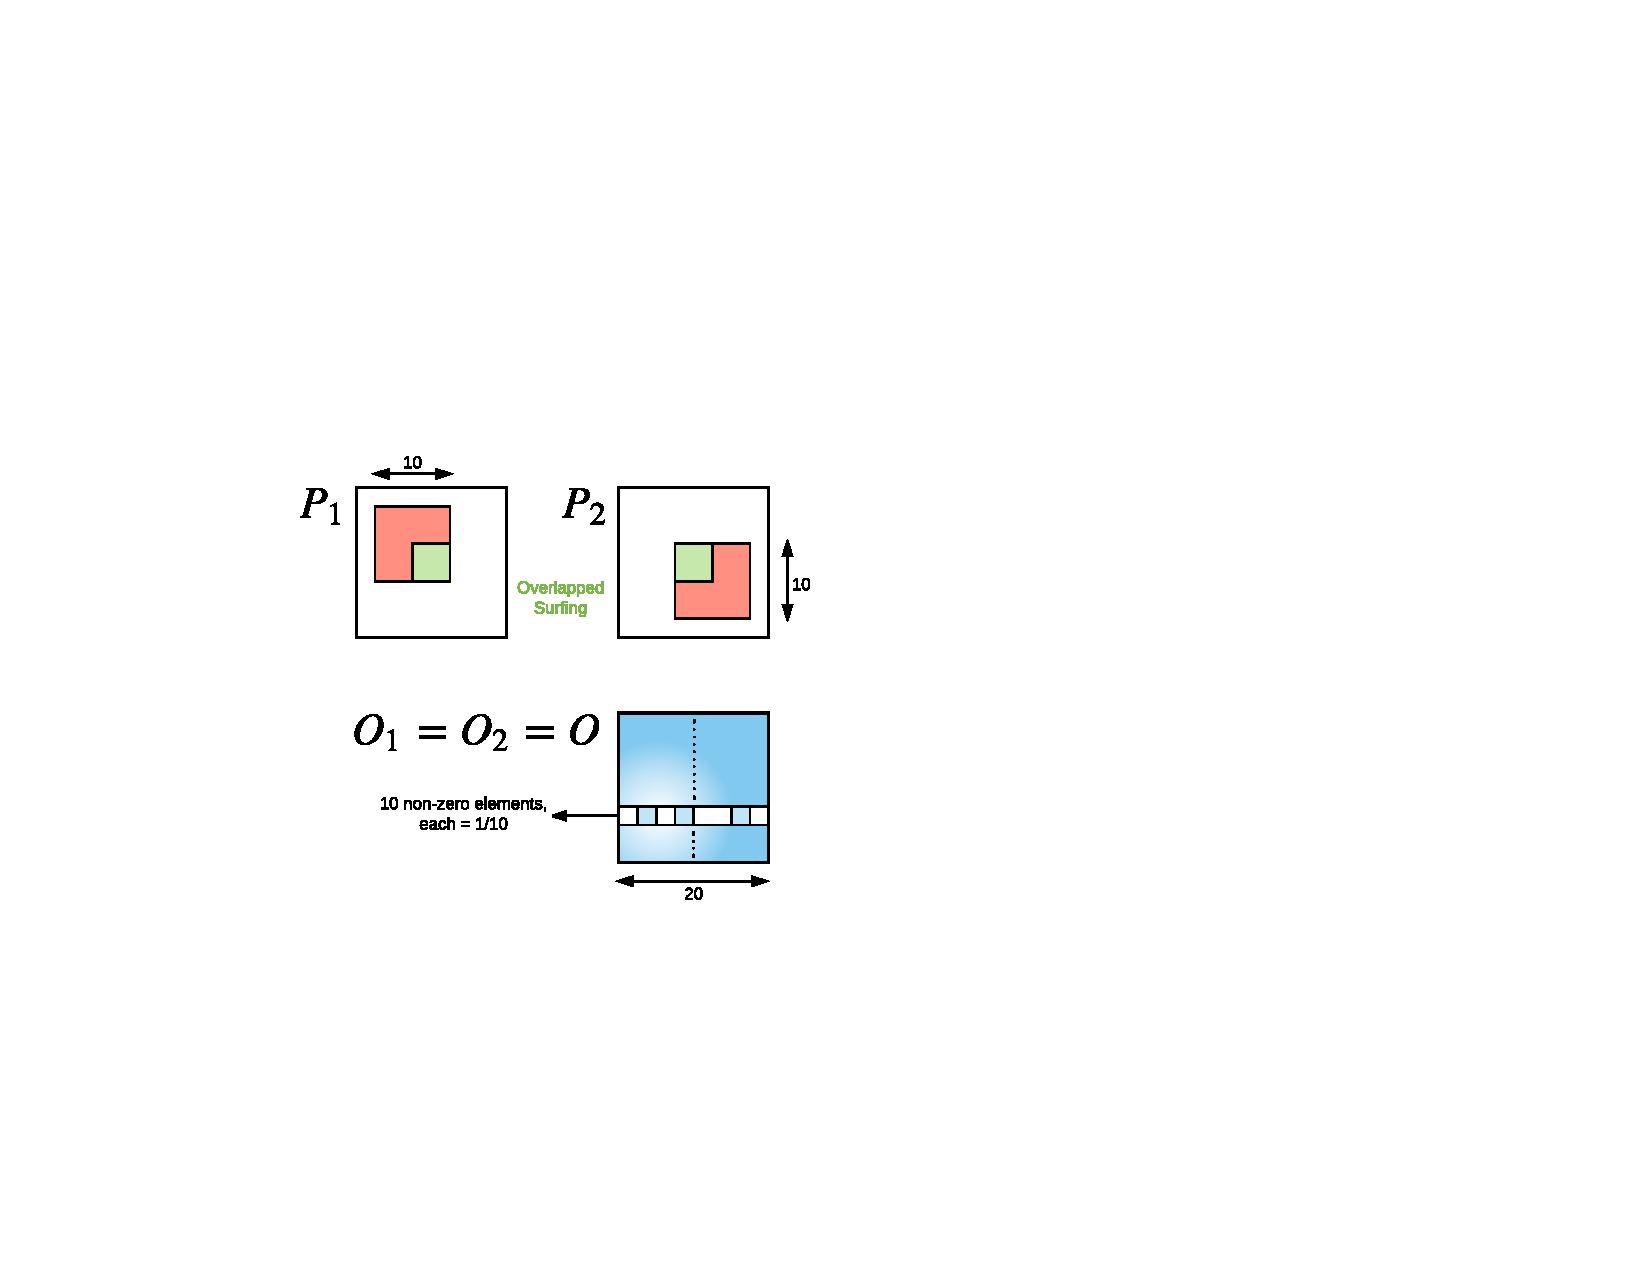
\includegraphics[width=\textwidth]{./img/case5-2}
			\caption{Case 5}
			\label{fig:case5}
		\end{subfigure}
		\caption{Illustration of the overlapped surfing without auxiliary block for $a = 10$ and $b = 20$.}\label{fig:osurf}
	\end{figure}
	
	
	\begin{figure}
		\centering
		\begin{subfigure}[b]{0.22\textwidth}
			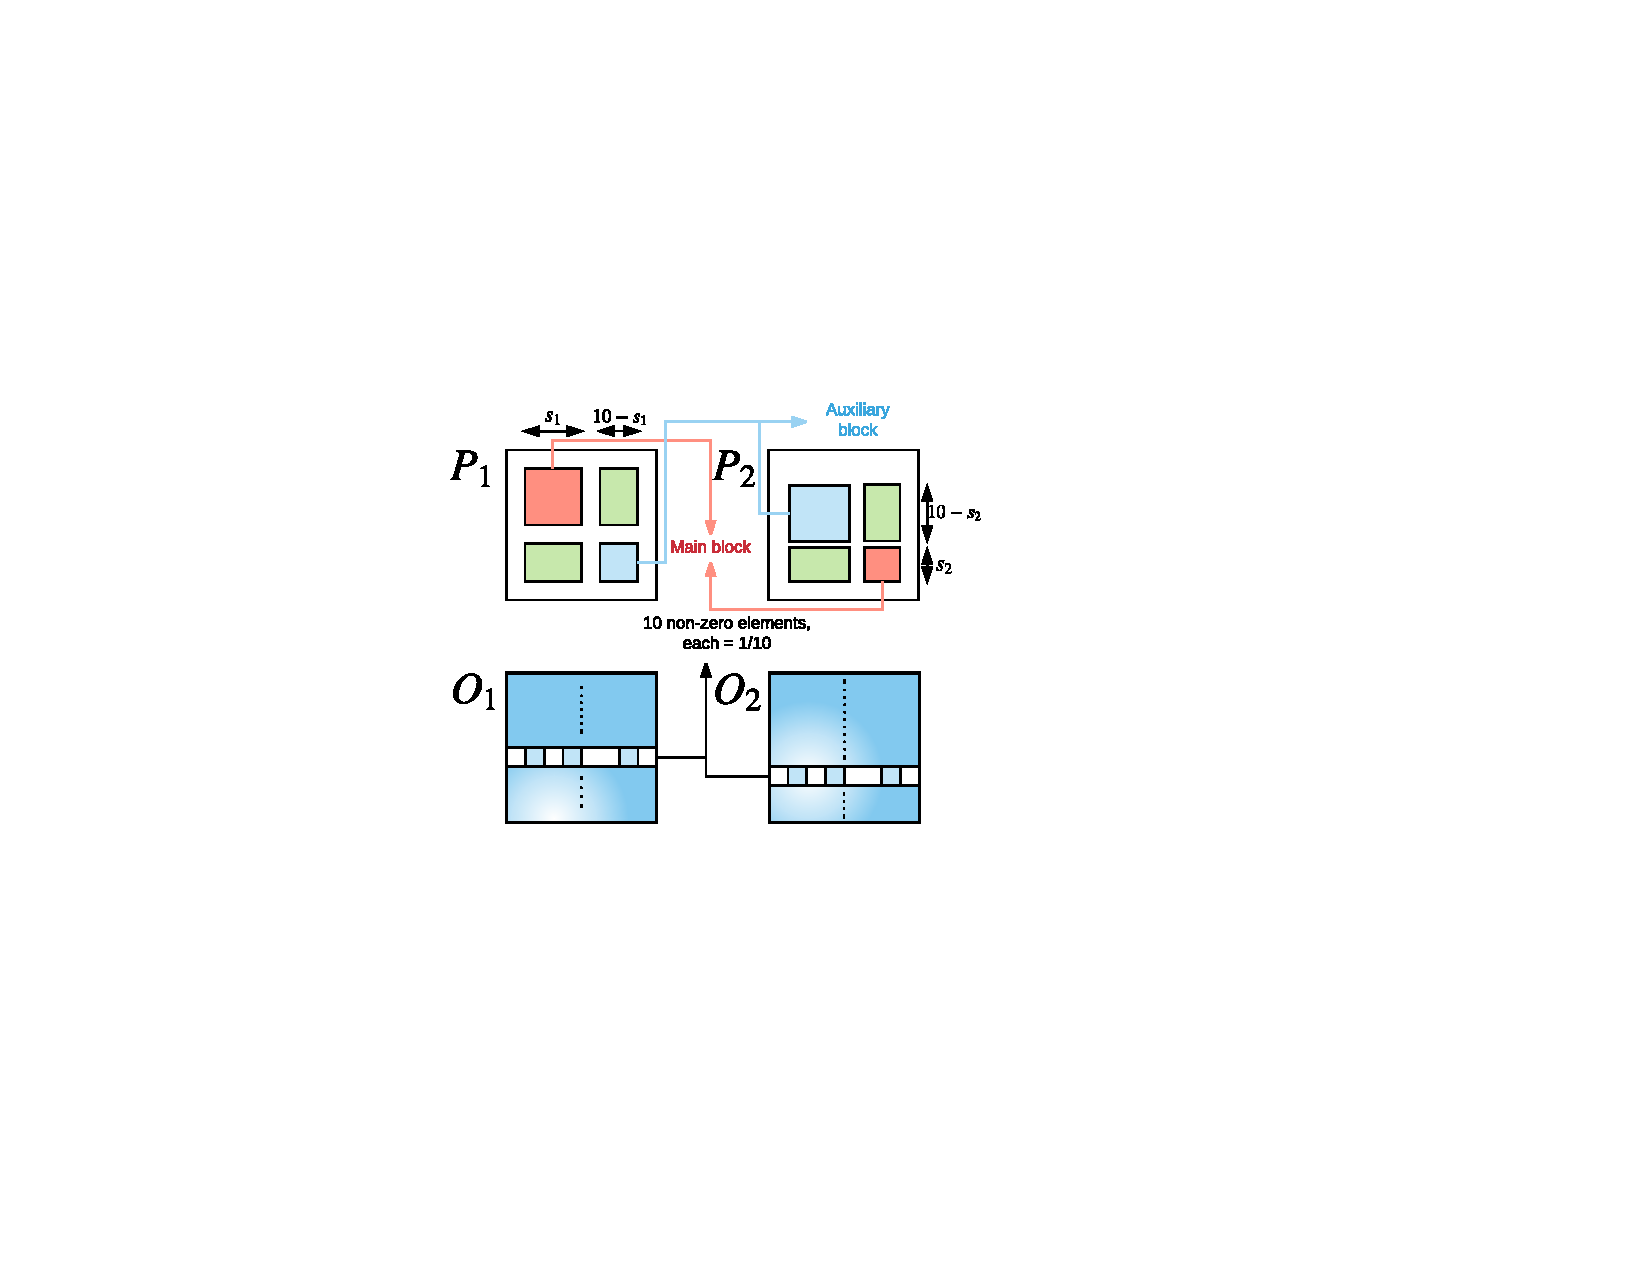
\includegraphics[width=\textwidth]{./img/case6-2}
			\caption{Case 6}
			\label{fig:case6}
		\end{subfigure}
		~ %add desired spacing between images, e. g. ~, \quad, \qquad, \hfill etc. 
		%(or a blank line to force the subFig onto a new line)
		\begin{subfigure}[b]{0.22\textwidth}
			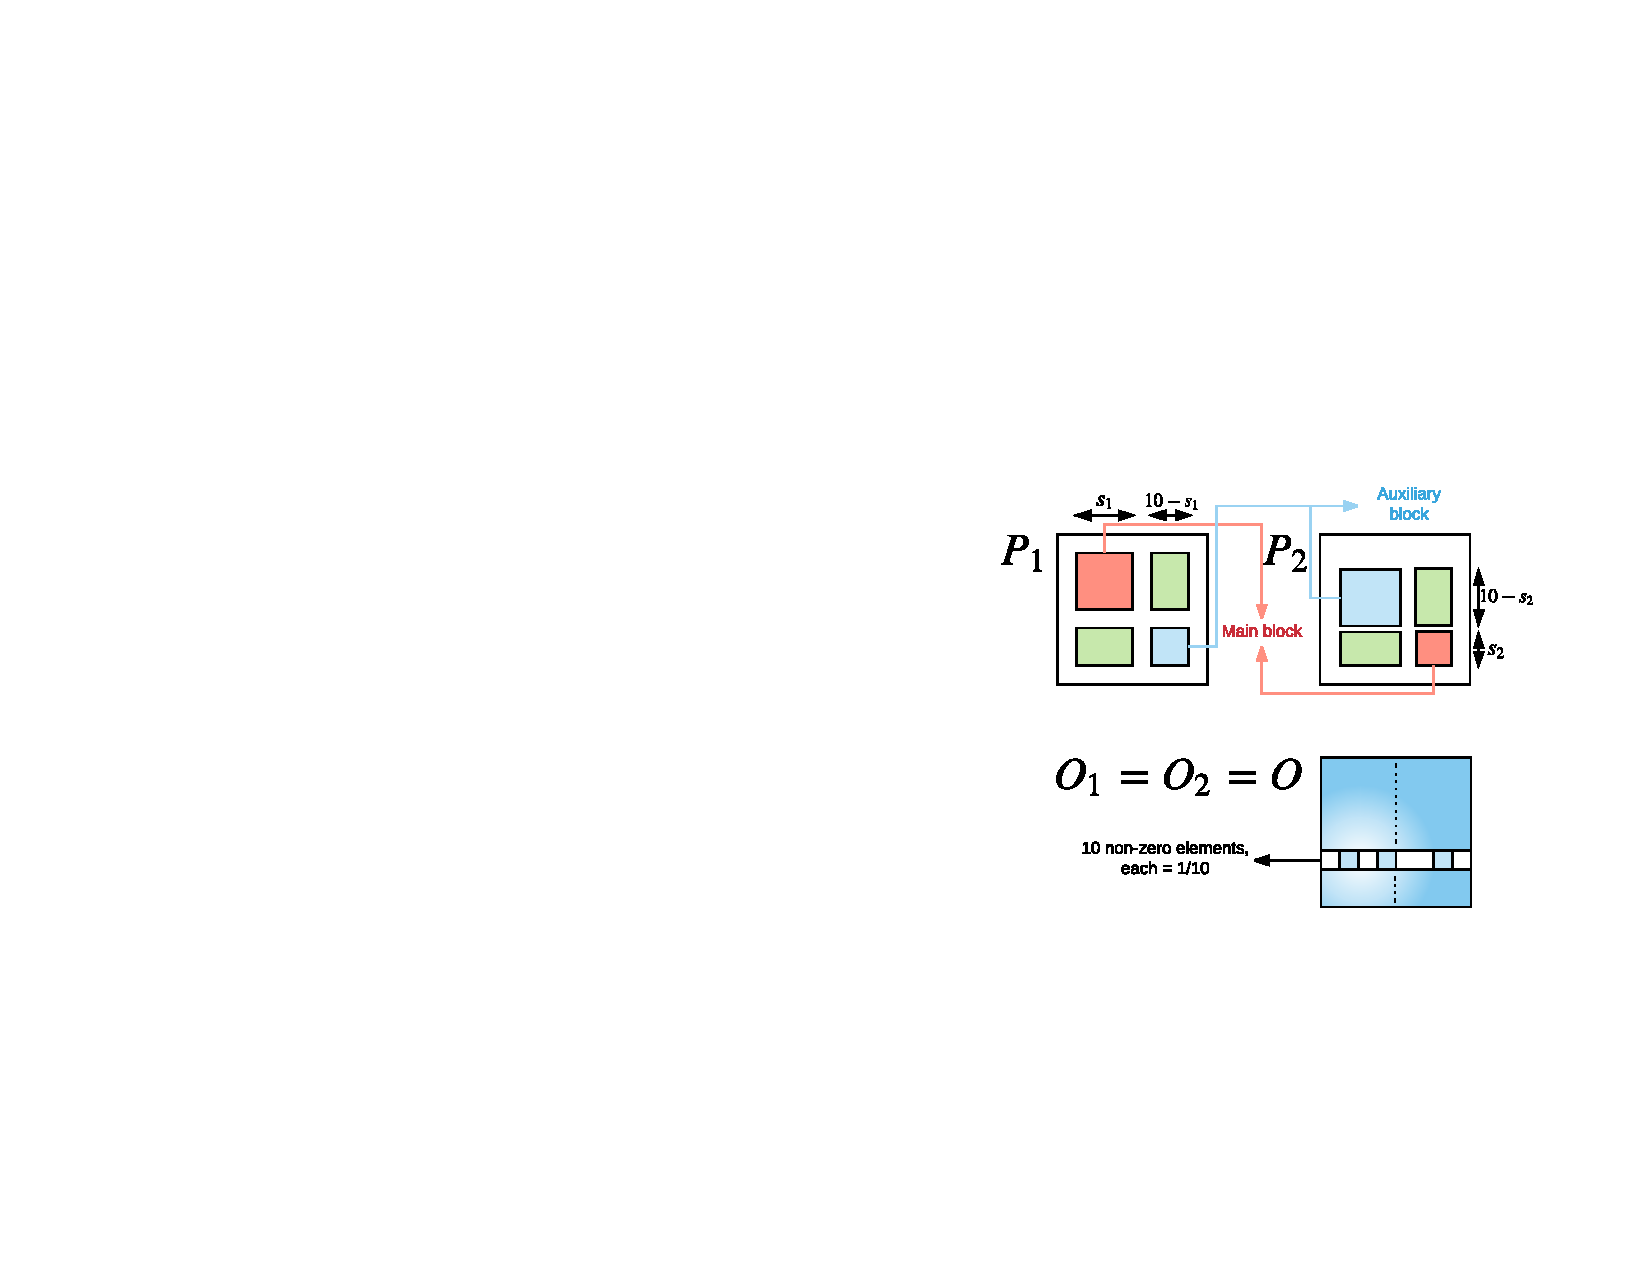
\includegraphics[width=\textwidth]{./img/case7-2}
			\caption{Case 7}
			\label{fig:case7}
		\end{subfigure}
		\caption{Illustration of the overlapped surfing with auxiliary block for $a = 10$ and $b = 20$.}\label{fig:osurfau}
	\end{figure}
	
	{\bf Probability Distributions:}
	\label{subsub:dist}
	Here we explain different distributions used in our synthetic generator:
	\begin{itemize}
		\item {Users shares vector $\aalpha$:} We fix $\aalpha$ to $(.4, .6)$.
		
		\item {Rows of user transition matrix $\A(u)$:} This is a diagonal dominant matrix, meaning that if user $u$ has submitted the current request $v(t)$ it is more probable that he submit the next request. 
		In this way, we capture the fact that because of the episodic nature of the request submission, close-by queries are more probable to come from a same user. 
		This has been exploited in the previous literature \cite{sigcomm}. Note that when instead of matrix $\A$ we only consider the vector $\aalpha$ we may not capture this realistic property of the data.
		For the toy example, we set $\alpha_{ii} = .5 + \frac{1}{2} \text{Uniform}(0,1)$ and $\forall i \neq j: \alpha_{ij} \propto (1 - \alpha_{ii}) \text{Uniform}(0,1)$
		
		\item {Rows of output matrix $\O_u(w)$:} As mentioned before, each row $\O_u(w)$ has $a$ non-zero elements with each with probability $1/a$.
		
		\item {Rows of page transition matrix $\P_u(w)$:} In a nutshell, we discretize a continuous Beta distribution with different parameters for each block and normalize the final vector.
		The distribution that we use for the (main) support is Beta(3+$\epsilon$,1+$\delta$) where $\epsilon$ and $\delta$ are random numbers from $[-1, 1]$. 
		For the distribution on the auxiliary support of the cases 6 and 7 above, we use Beta(2+$\epsilon$,2+$\delta$).
	\end{itemize}
	
	
	
	{\bf Discussion:}
	Table \ref{tab:as} shows the error of our method for all 7 cases of Section \ref{subsub:sparsity} for $a = 10$. 
	%Note that we report the result for both RNN and its variant LSTM. 
	
	\begin{table}
		\scriptsize  
		\centering
		\begin{tabular}{|c|c|c|c|c|c|c|c|c|}
			\hline
			\multicolumn{2}{|c|}{\bf \footnotesize Cases} & {\bf \footnotesize  1} & {\bf \footnotesize  2} & {\bf \footnotesize  3} & {\bf \footnotesize  4} & {\bf \footnotesize  5} & {\bf \footnotesize 6} & {\bf \footnotesize  7}  \\ 
			\hline  
			\multirow{2}{*}{$\aalpha$} & {\footnotesize  Mean} 	&  1 	& 1		&  .63 &  .70 & .62 &  .74& .65 \\ \cline{2-9}
			                           & {\footnotesize  Std} 	&  0 	& 0 	&  .02 &  .02 & .02 &  .05& .04 \\ \hline 
			\hline  
			\multirow{2}{*}{$A$}       & {\footnotesize  Mean} 	&  1 	& 1		&  .77 & .69 &  .67 & .82 & .78 \\ \cline{2-9}
			                           & {\footnotesize  Std} 	&  0 	& 0		&  .10 & .09 &  .08 & .09 & .16 \\ \hline 
		\end{tabular}
		\caption{Deinterleaving accuracy of= LSTM for different cases of the synthetic example when user transitions are determine by either of $\aalpha = [.4, .6]$ or random diagonally dominant $\A$.}
		\label{tab:as}
	\end{table}
	
	Each row is the average result for five instantiation of the model parameters $\O_u$ and $\P_u$. 
	The error of each instantiation (each row) is an average of 100 experiments. 
	Note that case 1 and 2 are trivial cases when both $\P$s and $\O$s are disjoint and LSTM perfectly dis-interleave. 
	Interestingly, performance in case 3 is much worse than cases 1 and 2, which confirms that in our model having disjoint output matrices is more important than disjoint surfing pattern. 
	Intuitively, this makes sense because the final request comes from the output matrices and if we have personalized outputs the deinterleaving should be easier. 
	Interestingly, beyond the trivial cases 1 and 2, case 6 has the best accuracy, probably because of personalized outputs and more complicated $\P_u$ for each user (composed of main and auxiliary block) makes the whole problem more separable. 
	
	%	This is by far better than what we have or even the literature of dis-interleaving has. 
	%	For (.4, .6) user share of requests, previous results (even in simple Markov chain interleaving not HsMM) are around at most .65 but here on the last experiment, we get about .78 accuracy. 
	%	Also, we are still measuring accuracy as the exact match between the inferred user and true users for all pages, which as we talked last time is a harsh criterion. 
	%	Vinod suggested that we should measure the accuracy only for the "popular enough" pages (We would appreciate if you can elaborate on this.)  
	
%	Since RNN and LSTM performances are very close and LSTM is more computationally demanding, in the following experiments we will only use RNN method. 
%	Note that when we use $\A$ instead of $\aalpha$ the error is smaller. 
%	This can be explained by the fact that with the diagonally dominated user transition matrix $\A$ neighbor requests in the resolver are more probable coming from a same user and this extra structure will help the algorithm to deinterleave more efficiently. 
%	
%	%	\subsubsection{Comparison with Viterbi Coding}
%	
%	
%	\subsubsection{Scalability}
%	In this set of synthetic experiment we increase the number of users and number of webpages report the performance of RNN-based deinterleaving methods. 
%
%	{\bf Scaling Users:}
%	\label{subsub:scalseusr}
%	In this set of experiments we increase the number of users and evaluate the performance of our RNN based method while changing the number of layers and hidden units of RNN. 
%	It is expected that adding more users makes the deinterleaving harder and therefore the error will increase. 
%	We perform two extreme experiments using each $\aalpha$ and $\A$ to control the user transition dynamics: 
%	
%	\begin{itemize}
%		\item User transition with $\aalpha$:
%		\begin{itemize}
%			\item $\aalpha$ is uniform over the users, i.e., $\alpha_i = \frac{1}{m}$. In this case, we expect deinterleaving to be very hard because there is no distinction between request generation rate of users. 
%			%			\item $\aalpha_i$ decreases geometrically in $i$, i.e., $\alpha_i = (1 - 2^{-m})^{-1} \times .5^i $
%		\end{itemize}
%		\item User transition with $\A$:
%		\begin{itemize}
%			%			\item $\alpha_{ii} = .5 + \frac{1}{2} \text{Uniform}(0,1)$ and $\forall i \neq j: \alpha_{ij} = (1 - \alpha_{ii}) \frac{1}{m - 1}$
%			\item $\alpha_{ii} = .5 + \frac{1}{2} \text{Uniform}(0,1)$ and $\alpha_{ij} = 
%			\begin{cases}
%			(1 - \alpha_{ii}) (1 - 2^{-m+1})^{-1} .5^j,     \quad j < i \\
%			(1 - \alpha_{ii}) (1 - 2^{-m+1})^{-1} .5^{j-1}, \quad j > i
%			\end{cases} 
%			$. 
%			Here, we have two properties that we hope to make deinterleaving easier. 
%			First, $\A$ is diagonally dominant which makes close-by queries more probable to come from same users. 
%			Also, the overall probability of picking users as active is non-uniform. 
%		\end{itemize}
%	\end{itemize} 
%	We perform experiment on $2, 5,$ and $10$ users and generate the synthetic data using the Case 6 of Section \ref{subsub:sparsity}. 
%	Maximum number of requests per page is limited to 5 and total number of pages $n$ is $1000$ while the support size of rows of matrices $a$ is $100$. 
%
%	
%%	\begin{figure}
%%		\centering
%%		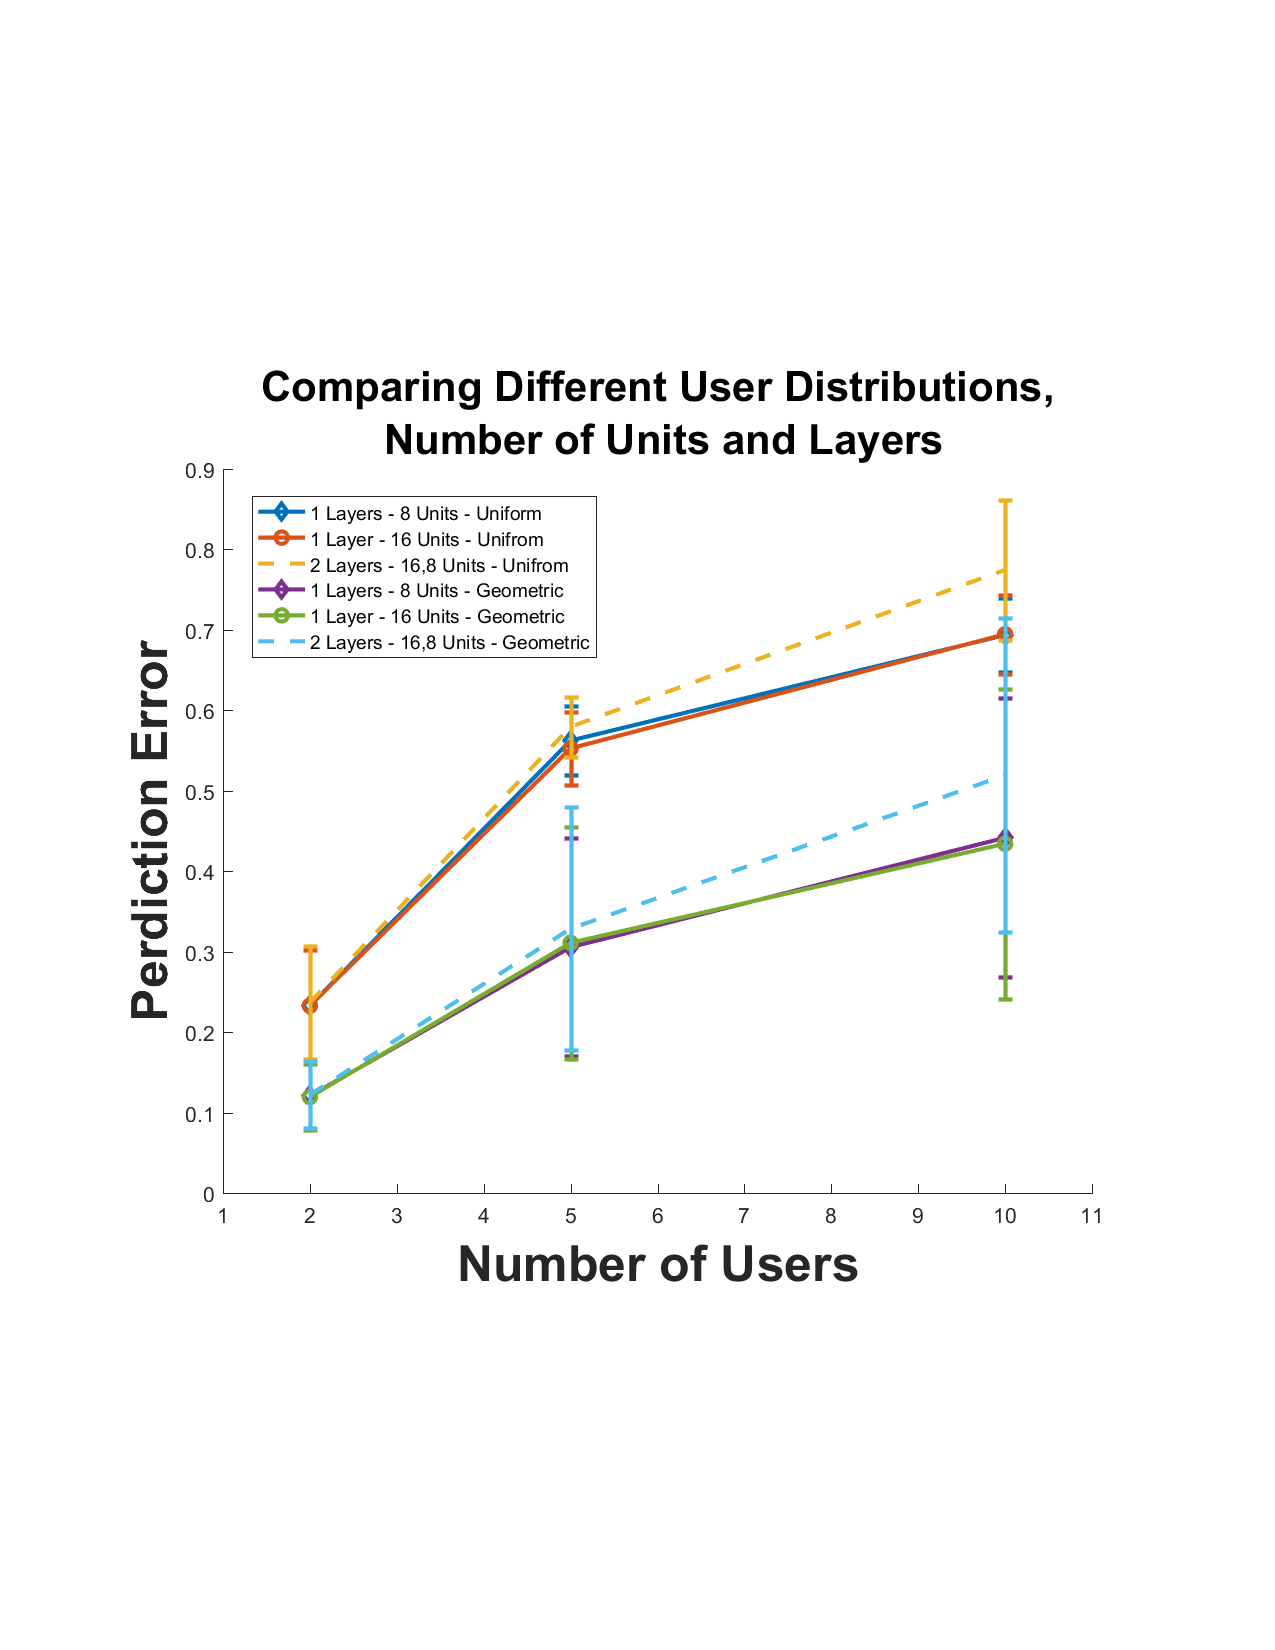
\includegraphics[width=.7\textwidth]{./img/users4}
%%		\caption{Comparing error for different user distributions, number of hidden layers and units.}
%%		\label{fig:user}
%%	\end{figure}
%	Fig \ref{fig:user} illustrates that deinterleaving becomes harder as we increase the number of users. 
%	But for the more realistic setup of user transition with matrix A even for 10 users we can reach 50\% accuracy.
%	Note that increasing the number of units is not helping the performance and increasing the layers overfits the data. 
%	
%	
%	{\bf Scaling Pages:}
%%	In this synthetic experiment we test the performance of our algorithm for two users with $\aalpha = [ .4, .6 ]$ while we increase the total number of pages $b$ linearly while keeping the support of each row of matrices as $a = n / 10$. 
%	In this synthetic experiment we test the performance of our algorithm for two users with matrix $\A$ generated as Section \ref{subsub:scalseusr} while we increase the total number of pages $b$ exponentially while keeping the support of each row of matrices as $a = n / 10$.
%	Maximum number of requests per page is limited to 5 and total number of pages $b$ is from the set $\{ 10^2, 10^3, 10^4, 10^5 \}$.
%	Based on the results of the user scalability experiment, we pick single layer RNN with 8 units. 
%	Fig \ref{fig:incpages} shows that as we increase the number of pages denterleaving becomes harder. 
%%	\begin{figure}
%%		\centering
%%		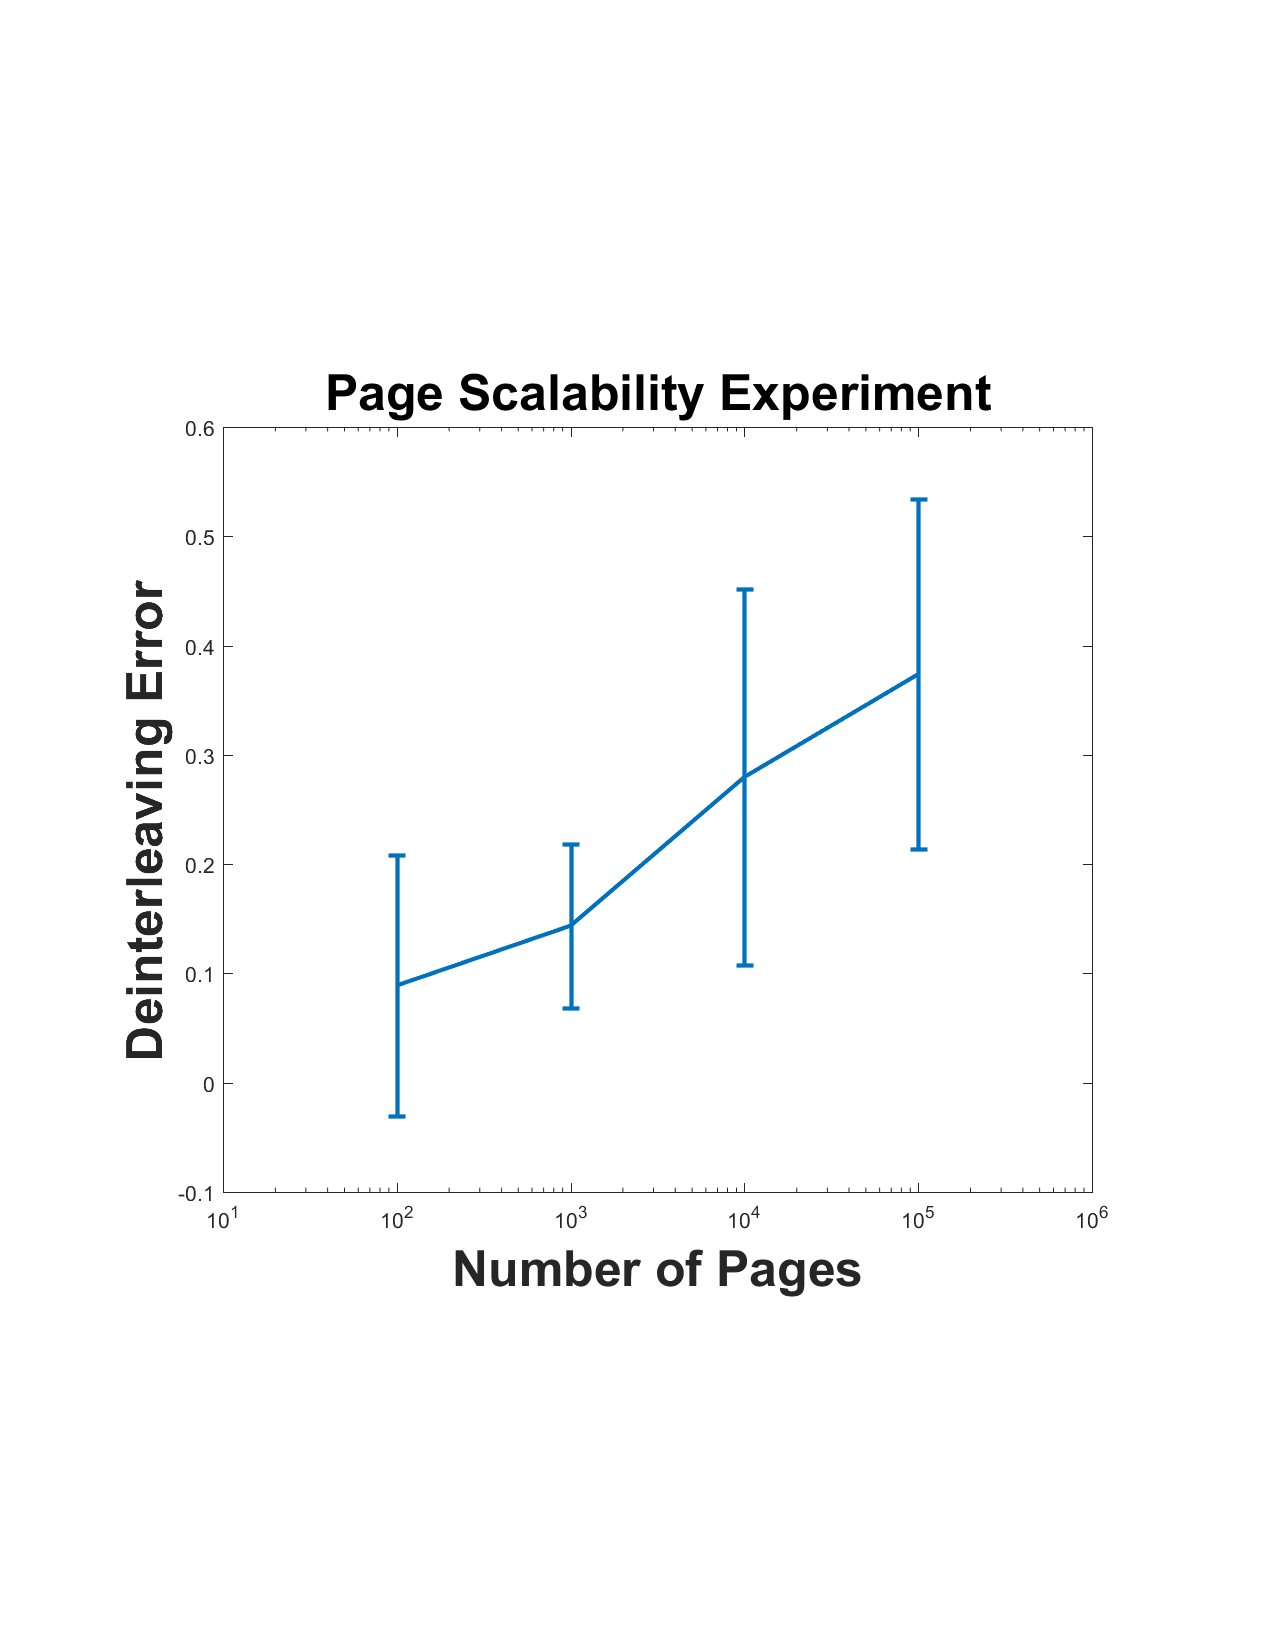
\includegraphics[width=.7\textwidth]{./img/incpages2}
%%		\caption{Scaling pages experiments.} 
%%		\label{fig:incpages}
%%	\end{figure}
%%	
%	\begin{figure}
%	\centering
%	\begin{subfigure}[b]{0.45\textwidth}
%		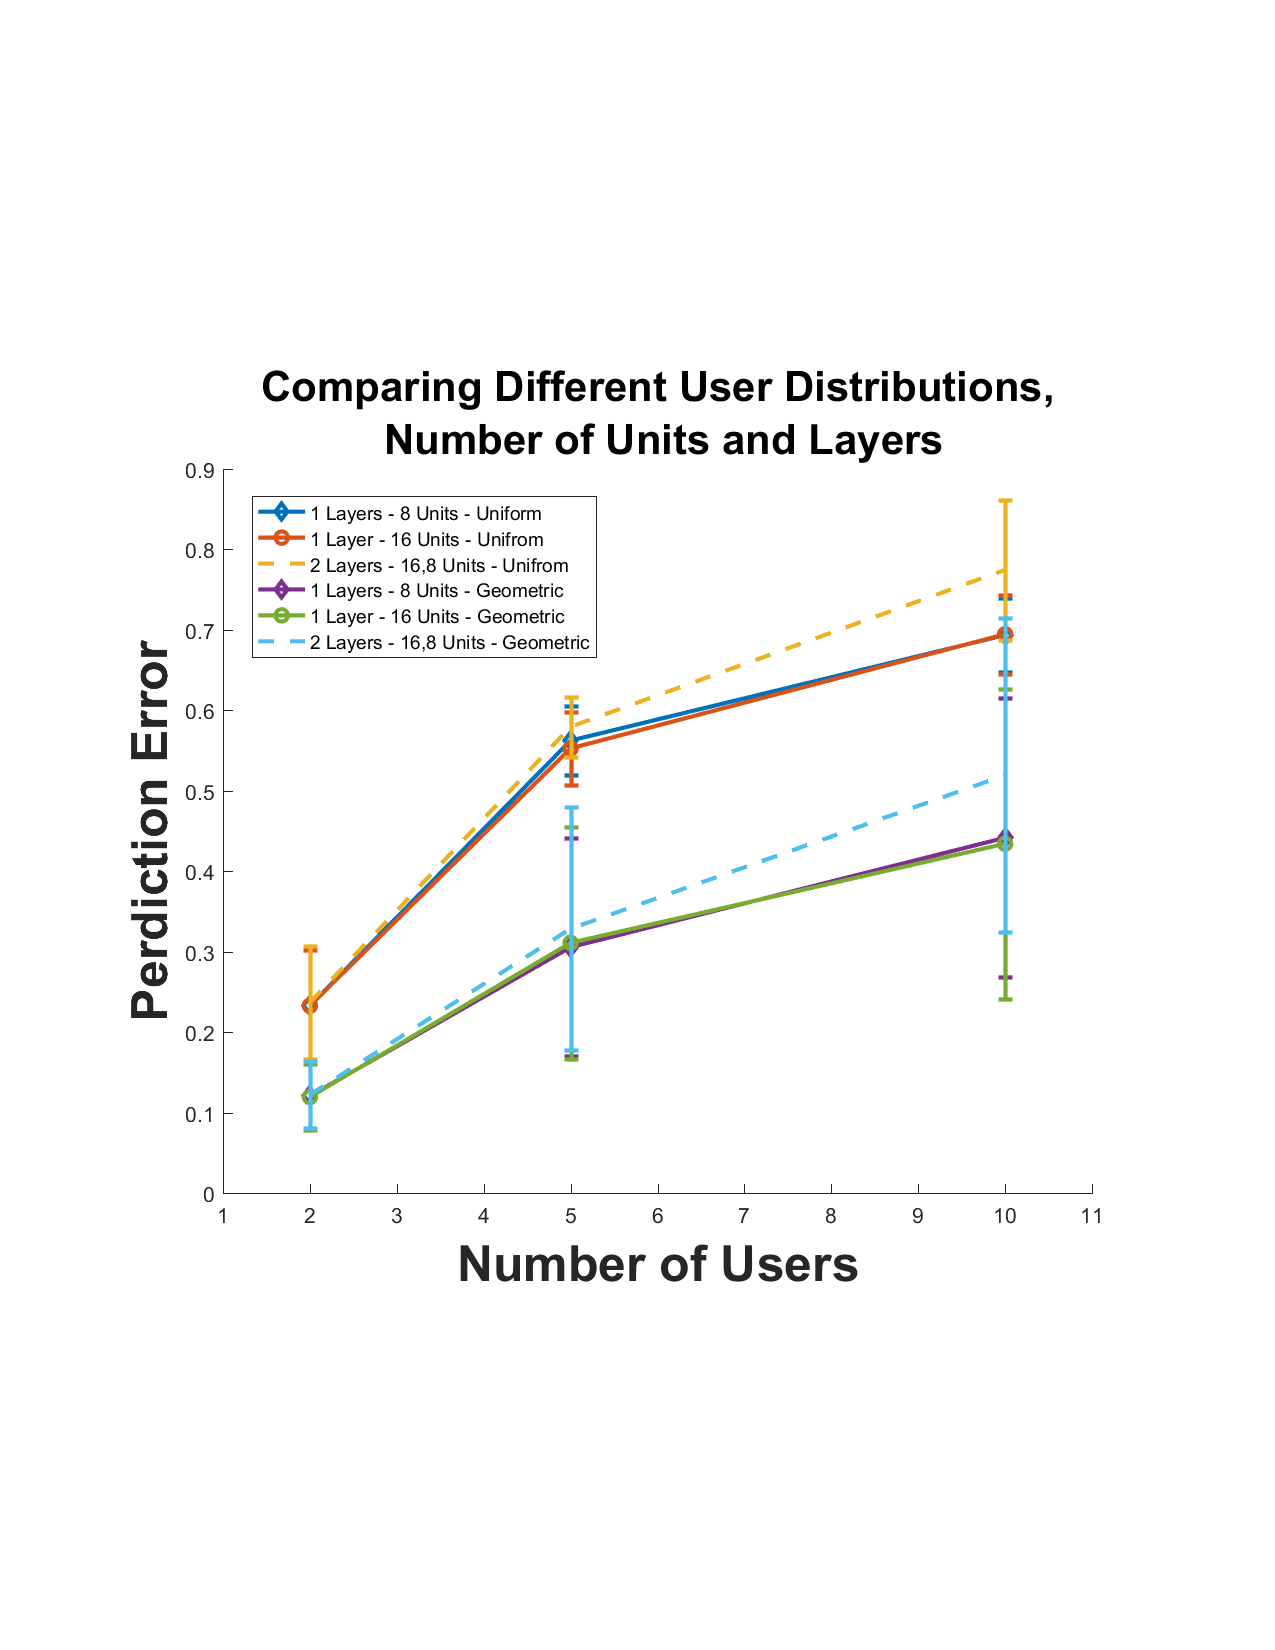
\includegraphics[width=\textwidth]{./img/users4}
%		\caption{Increasing number of users.}
%		\label{fig:user}
%	\end{subfigure}
%	~ %add desired spacing between images, e. g. ~, \quad, \qquad, \hfill etc. 
%	%(or a blank line to force the subFig onto a new line)
%	\begin{subfigure}[b]{0.45\textwidth}
%		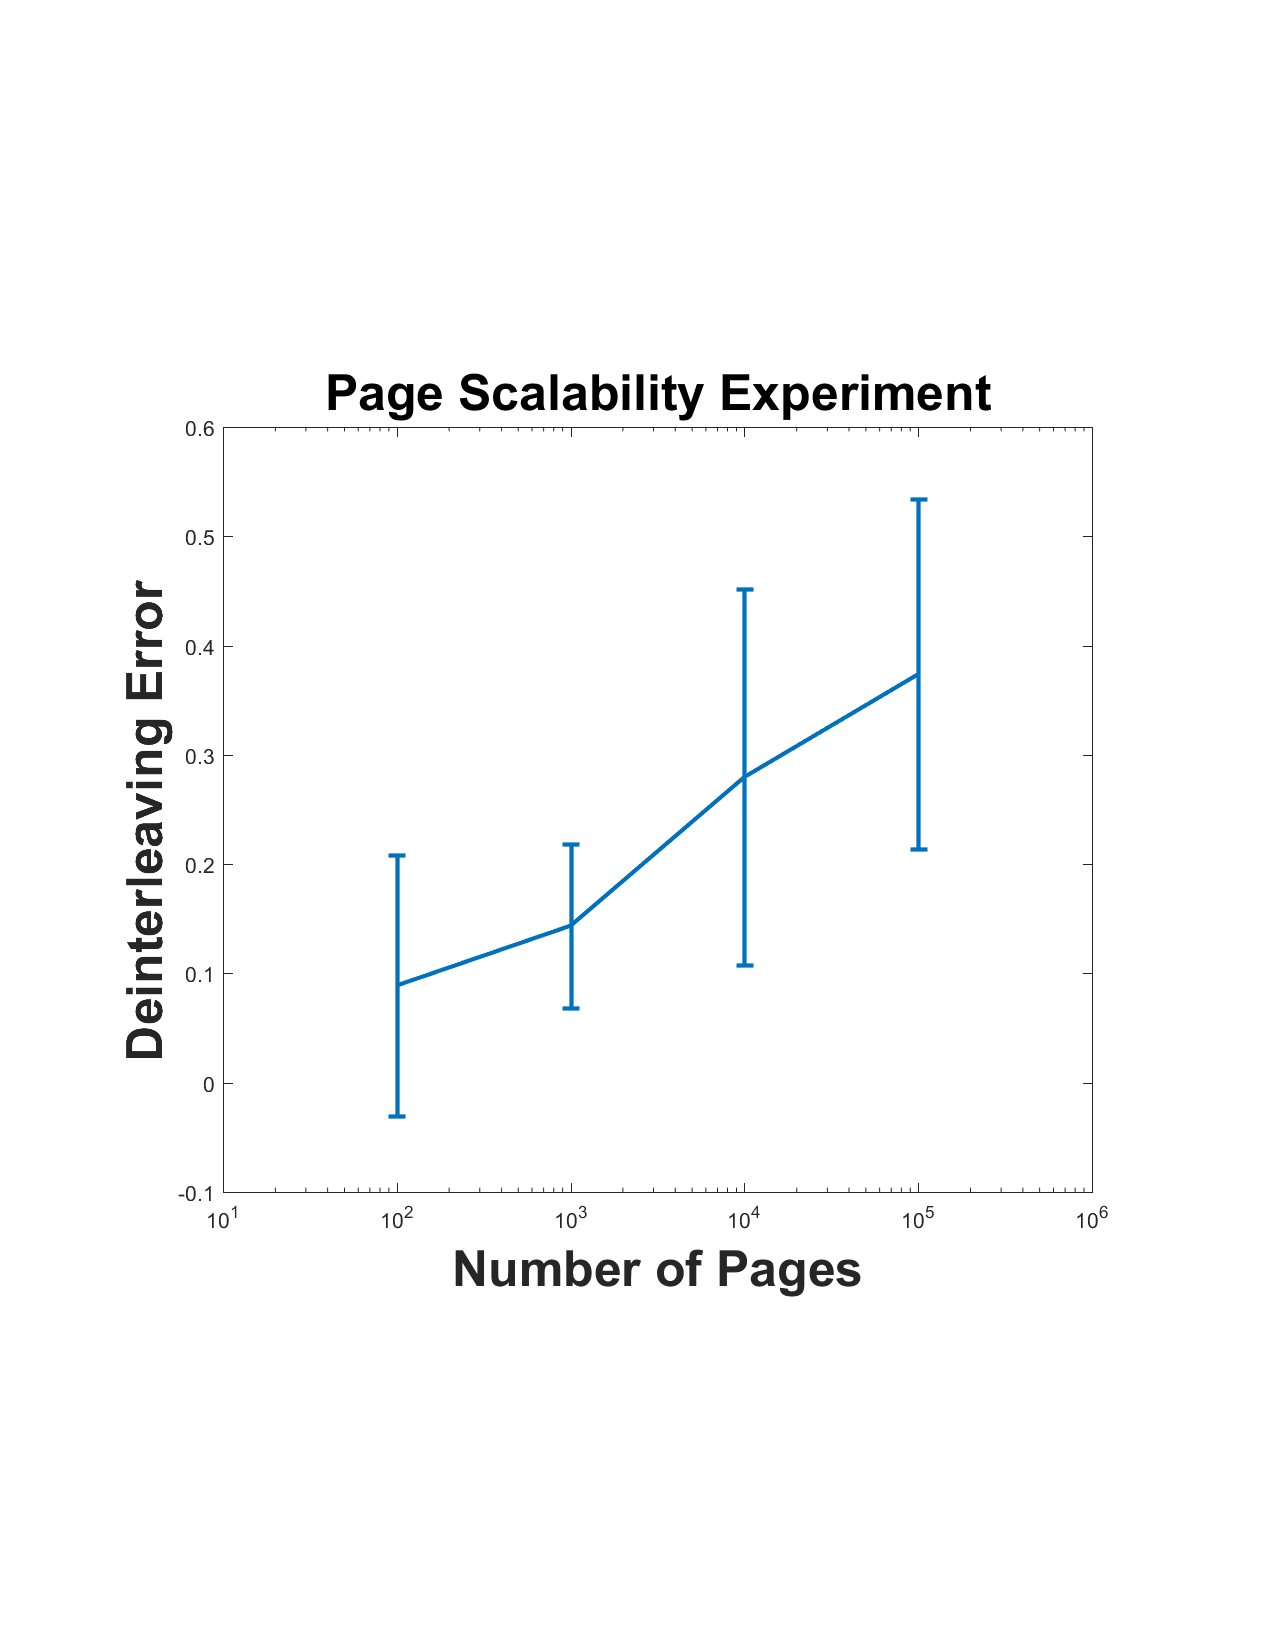
\includegraphics[width=\textwidth]{./img/incpages2}
%		\caption{Increasing number of pages.}
%		\label{fig:incpages}
%	\end{subfigure}
%	\caption{Scalability Experiment.}%\label{fig:osurfau}
%	\end{figure}
%	
%	\subsection{Real Data}
%	
%	
	
	
	
	%	Following are the results of the experiment in two separate setup. 
	%	First we assume that we know the parameters mentioned in Table \ref{tab:toy} and run the Viterbi algorithm and compute the accuracy for user, page, and state recovery.
	%	Next, we learn the parameters from the sequences using the Baum-Welch algorithm, then use the same sequence for Viterbi decoding and compute the accuracies. 
	%	
	%	\begin{figure}
	%		\centering
	%		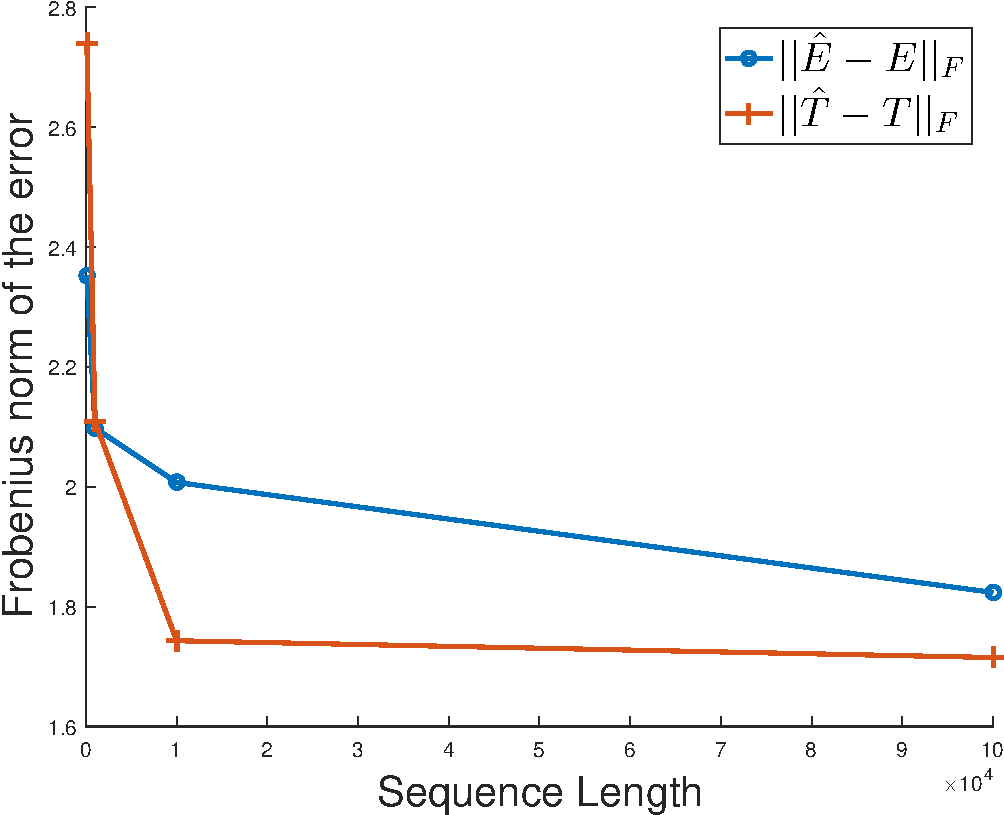
\includegraphics[scale=.4]{./img/frob-cropped}
	%		\caption{Error in learning transition matrix $T$ and emission matrix $E$ after 500 iterations of Baum-Welch algorithm (algorithm stops if the change in the log-likelihood of the observed sequence is less than 1e-6).}
	%		\label{fig:frob}
	%	\end{figure}	
	%	\begin{figure}
	%		\centering
	%		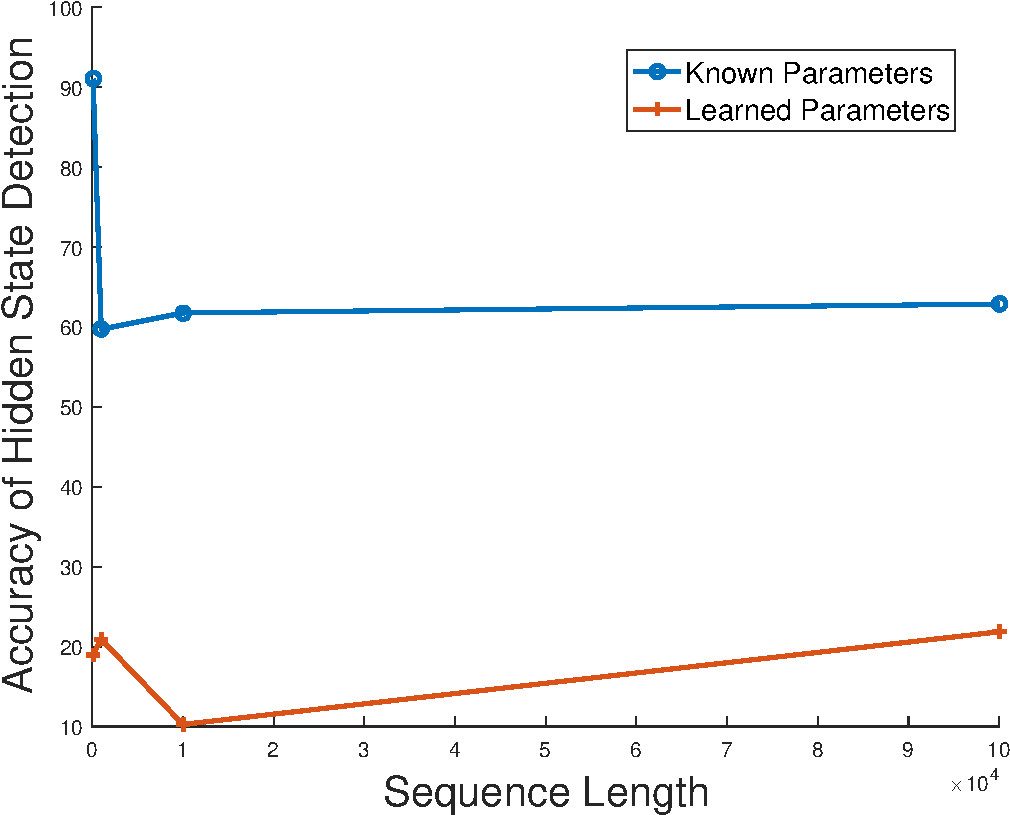
\includegraphics[scale=.4]{./img/states-cropped}
	%		\caption{Accuracy of hidden state detection using Viterbi for known and learned parameter. Obviously we do better when the parameters are known. Also for the unknown parameter as the number of samples increases, we learn the parameters more accurately \ref{fig:frob} which also improves Viterbi coding. The drop from 1000 to 10000 may be attributed to the fact that BW algorithm does not converge after 500 iterations when we go beyond 1000.}
	%		\label{fig:states}
	%	\end{figure}
	%	
	%	\begin{figure}
	%		\centering
	%		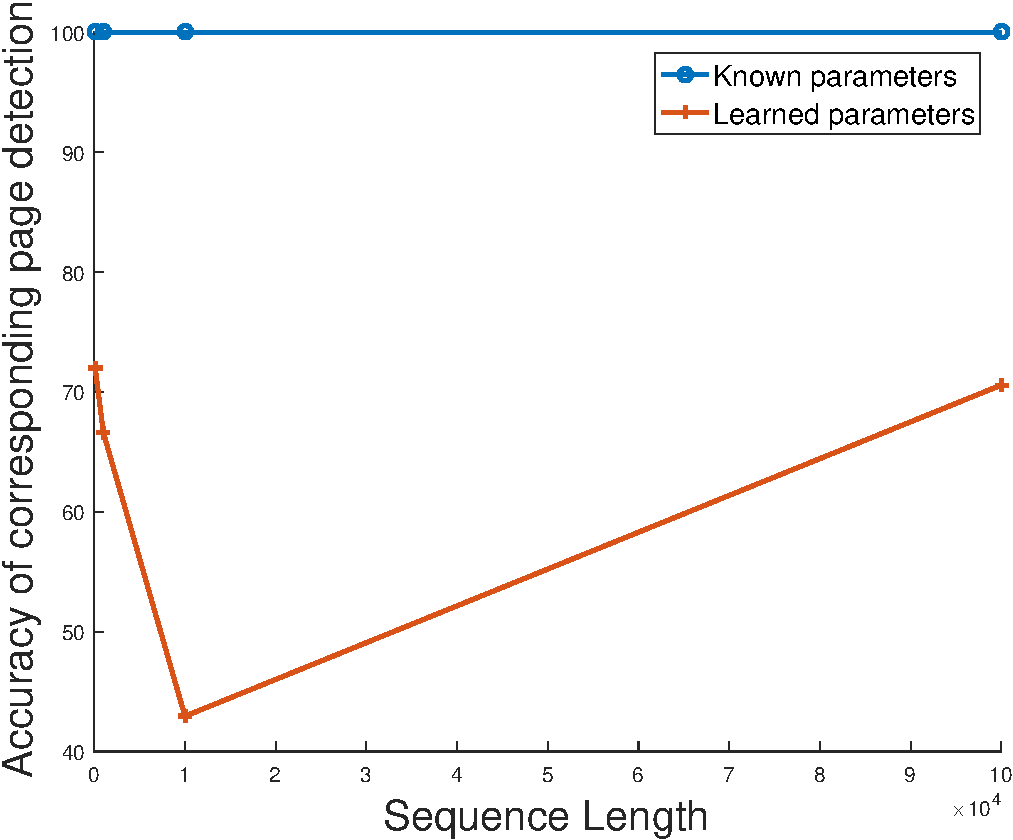
\includegraphics[scale=.4]{./img/pages-cropped}
	%		\caption{Accuracy of hidden page detection using Viterbi for known and learned parameter. We do prefect when the parameters are known. Also for the unknown parameter as the number of samples increases, we learn the parameters more accurately \ref{fig:frob} which also improves Viterbi coding. The drop from 1000 to 10000 may be attributed to the fact that BW algorithm does not converge after 500 iterations when we go beyond 1000. I think here we do better in comparison to user detection, because observation (visible sequence) depends completely on pages not users.}
	%		\label{fig:pages}
	%	\end{figure}
	%	
	%	\begin{figure}
	%		\centering
	%		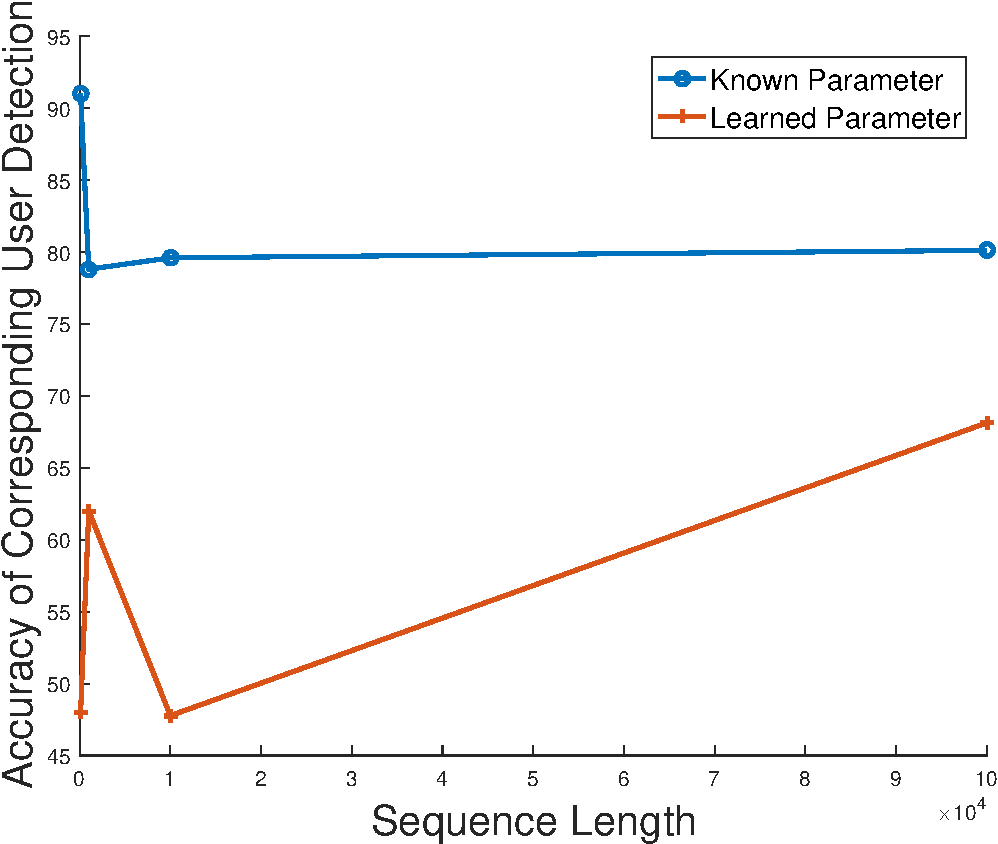
\includegraphics[scale=.5]{./img/users-cropped}
	%		\caption{Accuracy of hidden user detection (dis-interleaving solution) using Viterbi for known and learned parameter. We do around 80 percent with known parameters. Also for the unknown parameter as the number of samples increases, we learn the parameters more accurately \ref{fig:frob} which also improves Viterbi coding. The drop from 1000 to 10000 may be attributed to the fact that BW algorithm does not converge after 500 iterations when we go beyond 1000. I think as the interleaving paper mentioned, if we go from imbalanced $\aalpha = [0.2, 0.8]$ to more uniform $\aalpha$ accuracy drops.}
	%		\label{fig:users}
	%	\end{figure}
	%	
	
	%		
	%	Table \ref{tab:as} summarizes all of the assumptions.
	%	In the following we provide some details. 
	%	\begin{table}
	%		\centering
	%		\begin{tabular}{|c|l|}
	%			\hline
	%			Parameter & Value \\ 
	%			\hline  
	%			$m$ & 2 users \\ \hline
	%			$n$ & 20 pages \\ \hline
	%			$q$ & 1 request per page\\ \hline 
	%			$s$ & 3200 stats for the HMM\\ \hline 
	%			$t$ & 5000 sequence length of HMM (size of the resolver queue).\\ \hline 
	%			\hline 
	%			$\aalpha$ & The user's query generation probability is fixed to $[0.3, 0.7]$. \\ \hline 
	%			$\P_u \in \reals^{n \times n}$ & Entries drawn uniformly at random. \\ \hline 
	%			$p_w(d) \in \reals$ & Uniformly distributed, $d\sim U(1,2)$. \\ \hline 
	%			$\o_w(r) \in \reals^n$ & Drawn uniformly at random on all possible pages (domain names). \\ \hline 
	%		\end{tabular}
	%		\caption{Summary of the experiment setup.}
	%		\label{tab:as}
	%	\end{table}
	
	%	\noindent{\bf Generate Page Transition Matrix:}
	%	For each user we first generate a page transition matrix $\P_u$ completely at random. 
	%	
	%	\noindent{\bf Generate Duration Probability Distribution:}
	%	We assume that the number of requests per page is a uniform random variable over $[1, \texttt{NUM\_REQ}]$ interval.
	%	
	%	\noindent{\bf Generate HMM State Transition Matrix:}
	%	Since the hidden node has certain structure, state transitions are very restricted which makes the HMM transition matrix very sparse. 
	%	For example, from ``$01,00,02,10,05$'' we can go to either ``$01,00,02,10,04$'' or ``$00,00,01,10,05$'' and not any other state.
	%	Following our model we make the state transition matrix $\T\in \reals^{s\times s}$ from $\P_u\in \reals^{n\times n}$ and $p_w(d)$s.
	%		
	%	\noindent{\bf Generate Emission Matrix:}
	%	To build the emission probability matrix $\E \in \reals^{s\times p}$ of the HMM, for each hidden state $h$ we look at the active user $u$ and its current page $w_u$ and get the distribution $\o_{w_u}$ as the emission probability of that state. 
	%	
	%	\noindent{\bf Generate User Transition Vector:}
	%	We randomly generate a probability vector $\aalpha$. 
	
	
	%	\subsection{Viterbi Coding}
	%	The simplest algorithm in HMMs is the Viterbi coding algorithm. 
	%	Its running time for the dense transition matrix $\T \in \reals^{s\times s}$ and the observation sequence of length $t$ is $O(ts^2)$. 
	%	But our transition matrix is very sparse and we can reduce the running time to $O(t(s^2-z))$ where $z$ is the number of zeros in $\T$ which makes $s^2 - z$ the number of edges in the state transition graph. 
	%	
	%	In the following experiment we have $s= 3200$ states, which makes the running time in the order of $9 \times 10^6$ while only 7000 entries of $\T$ are non-zero. 
	%	Off-the-shelf HMM toolboxes are not exploiting the sparsity of the state transition matrix $\T$, so we need to write our own version of all of the required algorithm.
	%	We assume uniform distribution over all hidden states as the prior for first state in the Viterbi. 
	%	
	%	For the first round of the experiment we assume that the users' page transition matrices $\P_u$s, page emission probabilities $\o_w$s are given. 
	%	For the duration distribution $p_w(d)$ we use uniform distribution, over all possible requests. 
	%
	%	We are looking at correctly predicting the hyper-states of the HMM, pages, and user (the interleaving problem):
	%	\begin{table}[t]
	%		\centering
	%		\begin{tabular}{|l|l|l|}
	%			\hline 
	%			& Mean & Std \\ \hline 
	%			\hline
	%			State Recovery &  3.2000e-04 & 4.1312e-04\\ \hline  
	%			Page Recovery & 0.0521 & 0.0043\\ \hline
	%			User Recovery & 0.5001 & 0.0088\\ \hline
	%		\end{tabular}
	%		\caption{Summary of the experiment results for Viterbi algorithm with input of length 5000 generated from the model. The accuracy is the average over 10 runs of the experiment. Each run takes about 45 min.}
	%		\label{tab:as}
	%	\end{table}
	%	
	%	As you see the results are not good. 
	%	My current thinking:
	%	\begin{itemize}
	%		\item Maybe uniform distribution for all parameters makes it hard to infer the model. 
	%		\item Is the sequence length important? Is it possible to get better results with longer sequence? or this is only true for the parameter learning's sample complexity. 
	%		\item At first I was thinking that since the emission probability is only depend on the page and is independent of the user, from such observation we can not recover users correctly. But based on the results we can't recover  the pages either. Note that the page recovery is harder since there are 20 of them compare to 2 possible users. 
	%	\end{itemize}
	
	%	\begin{table}
	%		{\footnotesize
	%		\begin{tabular}{|c|c||c|l|}
	%			Python var& Math var& Explanation & Size \\ 
	%			\hline 
	%			\texttt{\footnotesize stateList} & $-$ & {\footnotesize A list that maps state ID to the state code} & $s(2m+1)c$ \\
	%			\texttt{\footnotesize pageTransitionList} & $\{\P_u\}_{u=1}^m, \P_u \in \reals^{n\times n}$ & {\footnotesize $[\P_u]_{w'w}$ is the probability of user $u$ jumps from page $w'$} to $w$ & $mn^m$ \\
	%			\texttt{\footnotesize userTransitionVector} & $\alpha \in \reals^m$ & {\footnotesize $\alpha_u$ determines the probability of the $u$th user} & $m$ \\
	%			\texttt{emissionProb} & $\E \in \reals^{n\times n}$ & {$\alpha_u$ determines the probability of the $u$th user} & $m$
	%		\end{tabular}
	%		}
	%	\end{table}
	%	
	%	\begin{table}
	%		{\footnotesize
	%			\begin{tabular}{|c||c|l|}
	%				Math var& Explanation & Size \\ 
	%				\hline 
	%				$-$ & {\footnotesize A list that maps state ID to the state code} & $s(2m+1)c$ \\
	%				$\{\P_u\}_{u=1}^m, \P_u \in \reals^{n\times n}$ & {\footnotesize $[\P_u]_{w'w}$ is the probability of user $u$ jumps from page $w'$} to $w$ & $mn^m$ \\
	%				$\alpha \in \reals^m$ & {\footnotesize $\alpha_u$ determines the probability of the $u$th user} & $m$ \\
	%				$\E \in \reals^{n\times n}$ & {$\alpha_u$ determines the probability of the $u$th user} & $m$
	%			\end{tabular}
	%		}
	%	\end{table}

 
	
\bibliographystyle{plain}
\bibliography{main}



\end{document}
